\documentclass{beamer}

\usepackage[T1]{fontenc}
\usepackage[utf8]{inputenc}
\usepackage[english]{babel}
\usepackage{lmodern}
\usepackage{tikz}
\usepackage{booktabs}
\usepackage{amsmath}
\usepackage{amssymb}
\usepackage{algorithm}
\usepackage{algpseudocode}
\usepackage{tabularx}
\usepackage{graphicx}
\usepackage{xcolor}
\usepackage{adjustbox}
\usepackage{animate}
\usepackage{listings}
\usepackage{mathtools}
\usetikzlibrary{positioning,calc,decorations.pathreplacing,shapes.geometric,arrows.meta}



% ----------------------------------------
%  ENVIRONMENT SETUP
% ----------------------------------------

\newenvironment{secframe}
  {\begin{frame}{\insertsection}} % ouverture : crée une frame avec le titre de la section courante
  {\end{frame}} 

% ----------------------------------------


% Use Unipd as theme, with options:
% - pageofpages: define the separation symbol of the footer page of pages (e.g.: of, di, /, default: of)
% - logo: position another logo near the Unipd logo in the title page (e.g. department logo), passing the second logo path as option 
% Use the environment lastframe to add the endframe text
\usetheme[pageofpages=of]{Unipd}

\title{Differential Equations Simulator using
NFTMs}
\subtitle{Supervise: Akash Malhotra}
\author[Lucia Fernandez Sanchez, Alexandra Perruchot-Triboulet Rodriguez, Samuel Chapuis]{L.~Fernandez Sanchez \and A.~Perruchot-Triboulet Rodriguez \and S.~Chapuis}

\date{\today}

% The next block of commands puts the table of contents at the beginning of each section and highlights the current section
\AtBeginSection[]
{
  \begin{frame}
    \frametitle{Table of Contents}
    \setbeamerfont{section in toc}{size=\small}
    \tableofcontents[currentsection]
  \end{frame}
}



\begin{document}

% Make the title page
\frame{\titlepage}
\section{Motivation}

\begin{secframe}

  \vspace{-2.6mm}
\begin{figure}[t]
\centering

\adjustbox{center}{%
  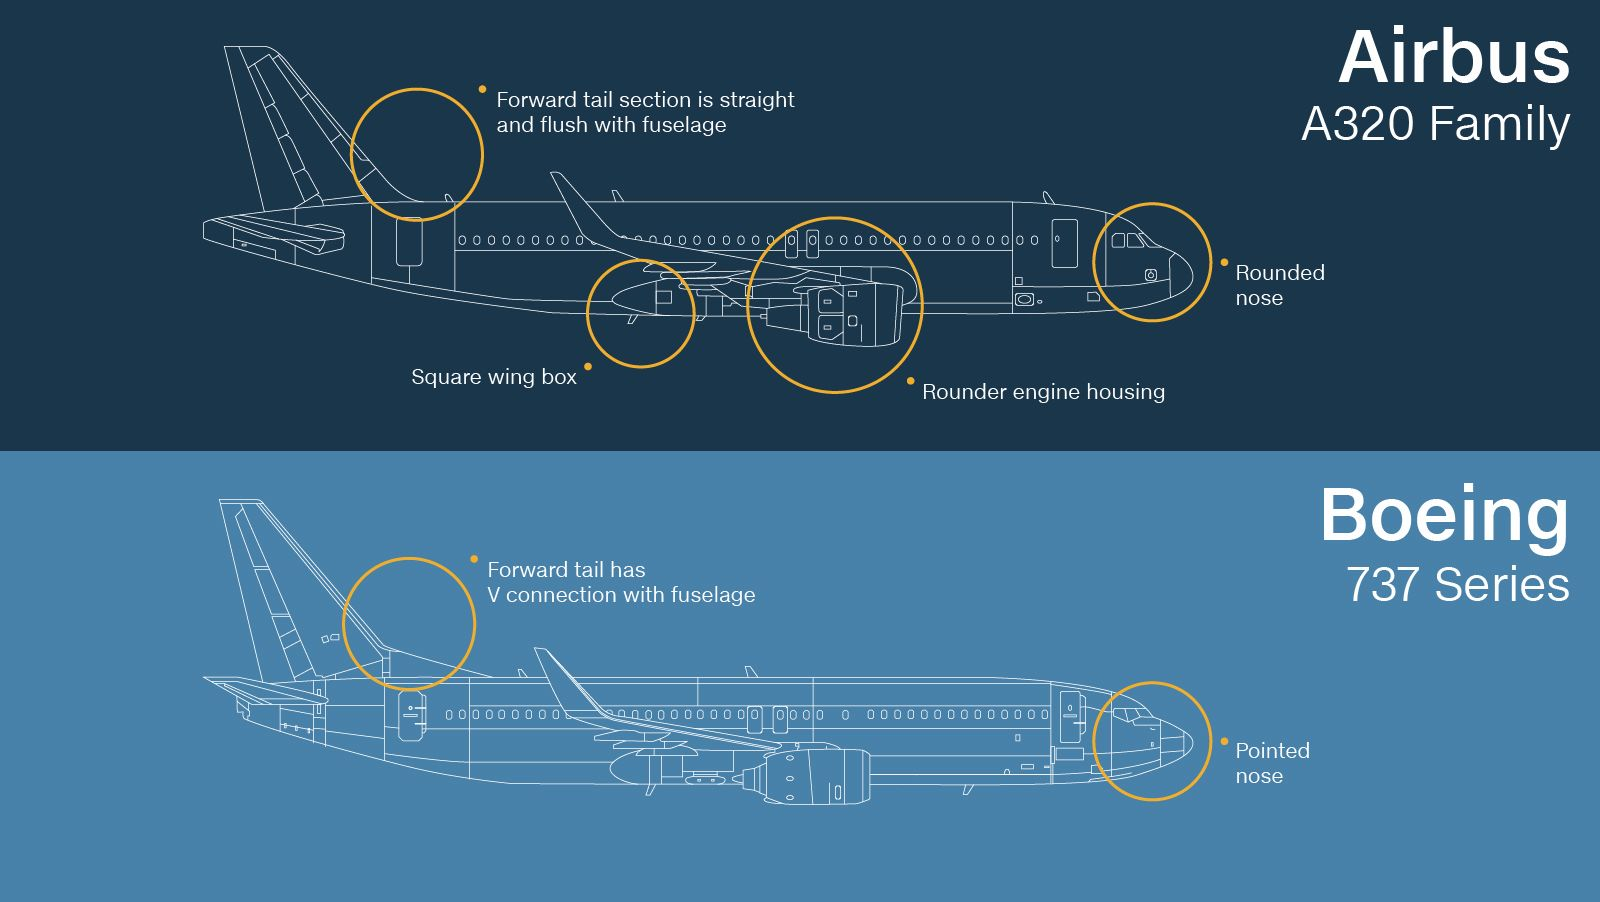
\includegraphics[width=1.03\paperwidth, height=0.85\paperheight]{images/illustration/airbusVSboeing.jpg}
}
\end{figure}

\end{secframe}

\begin{secframe}
  \textcolor{red_unipd}{\Large CFD over foil}

  \begin{block}{Modern Computational Fluid Dynamics (CFD) simulations}
    \begin{itemize}
      \item Essential for aerospace design, weather forecasting, and more
      \item Computationally expensive, especially for turbulent flows
    \end{itemize}
  \end{block}


  \begin{figure}
    \centering
    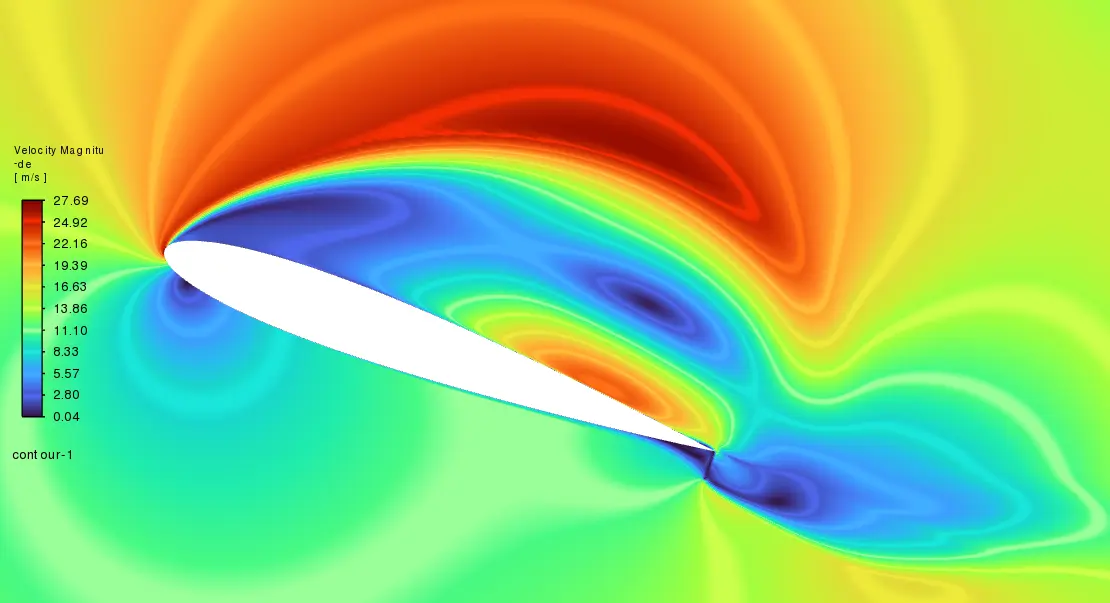
\includegraphics[width=0.9\textwidth]{images/illustration/foil.png}
  \end{figure}

\end{secframe}


\begin{secframe}
  \textcolor{red_unipd}{\Large Real thermal application}

  \begin{block}{Real thermal application}
    Thermal application from Samuel's master thesis
  \end{block}

  \begin{figure}
    \centering
    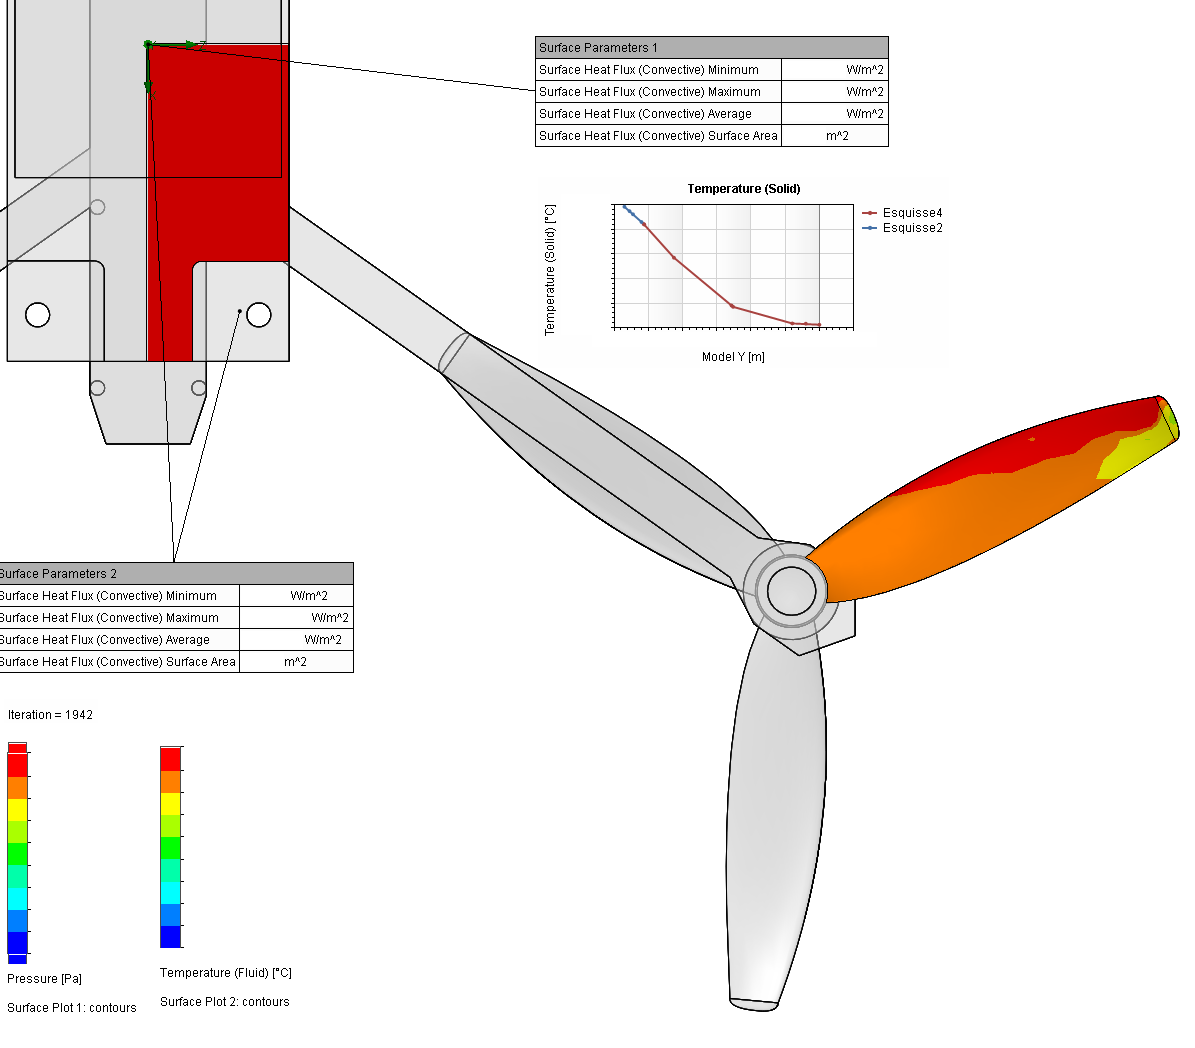
\includegraphics[width=0.9\textwidth]{images/illustration/BaseLine.png}
  \end{figure}

\end{secframe}


\begin{secframe}
  \textcolor{red_unipd}{\Large Kolmogorov energy cascade}
  \vspace{0.6em}

  \begin{figure}
    \centering
    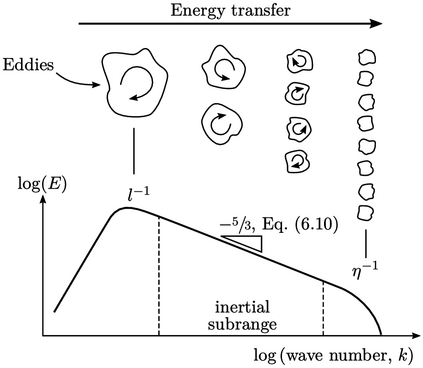
\includegraphics[width=0.7\textwidth]{images/illustration/kolmogorov.png}
  \end{figure}

\end{secframe}
 % Samuel
\section{State Of the Art}

\begin{frame}{Implementation}
    \small
    \textcolor{red_unipd}{\Large Retrieve Data}
    \vspace{0.5em}

    \begin{columns}[T]
        \begin{column}{0.48\textwidth}
            \begin{block}{ETL}
                Retrieves papers from Springer API, matches their ISSNs with a pre-loaded database of 22 journals, and augments each paper with its journal's h-index.
            \end{block}
        \end{column}
        \begin{column}{0.48\textwidth}
            \begin{block}{dataVis}
                Loads the augmented paper data, filters papers with valid h-indices, generates statistical summaries and 4 visualizations, and exports results to CSV/Excel.
            \end{block}
        \end{column}
    \end{columns}

\end{frame}

\begin{frame}{Implementation}
    \small
    \textcolor{red_unipd}{\Large H-Index Statistics}
    \vspace{0.5em}

    \begin{columns}[T]
        \begin{column}{0.25\textwidth}
            \begin{block}{Statistics}
                \begin{itemize}
                    \item Papers with h-index: 22
                    \item Papers without h-index: 3
                \end{itemize}
            \end{block}
        \end{column}
        \begin{column}{0.73\textwidth}
            \begin{figure}
                \centering
                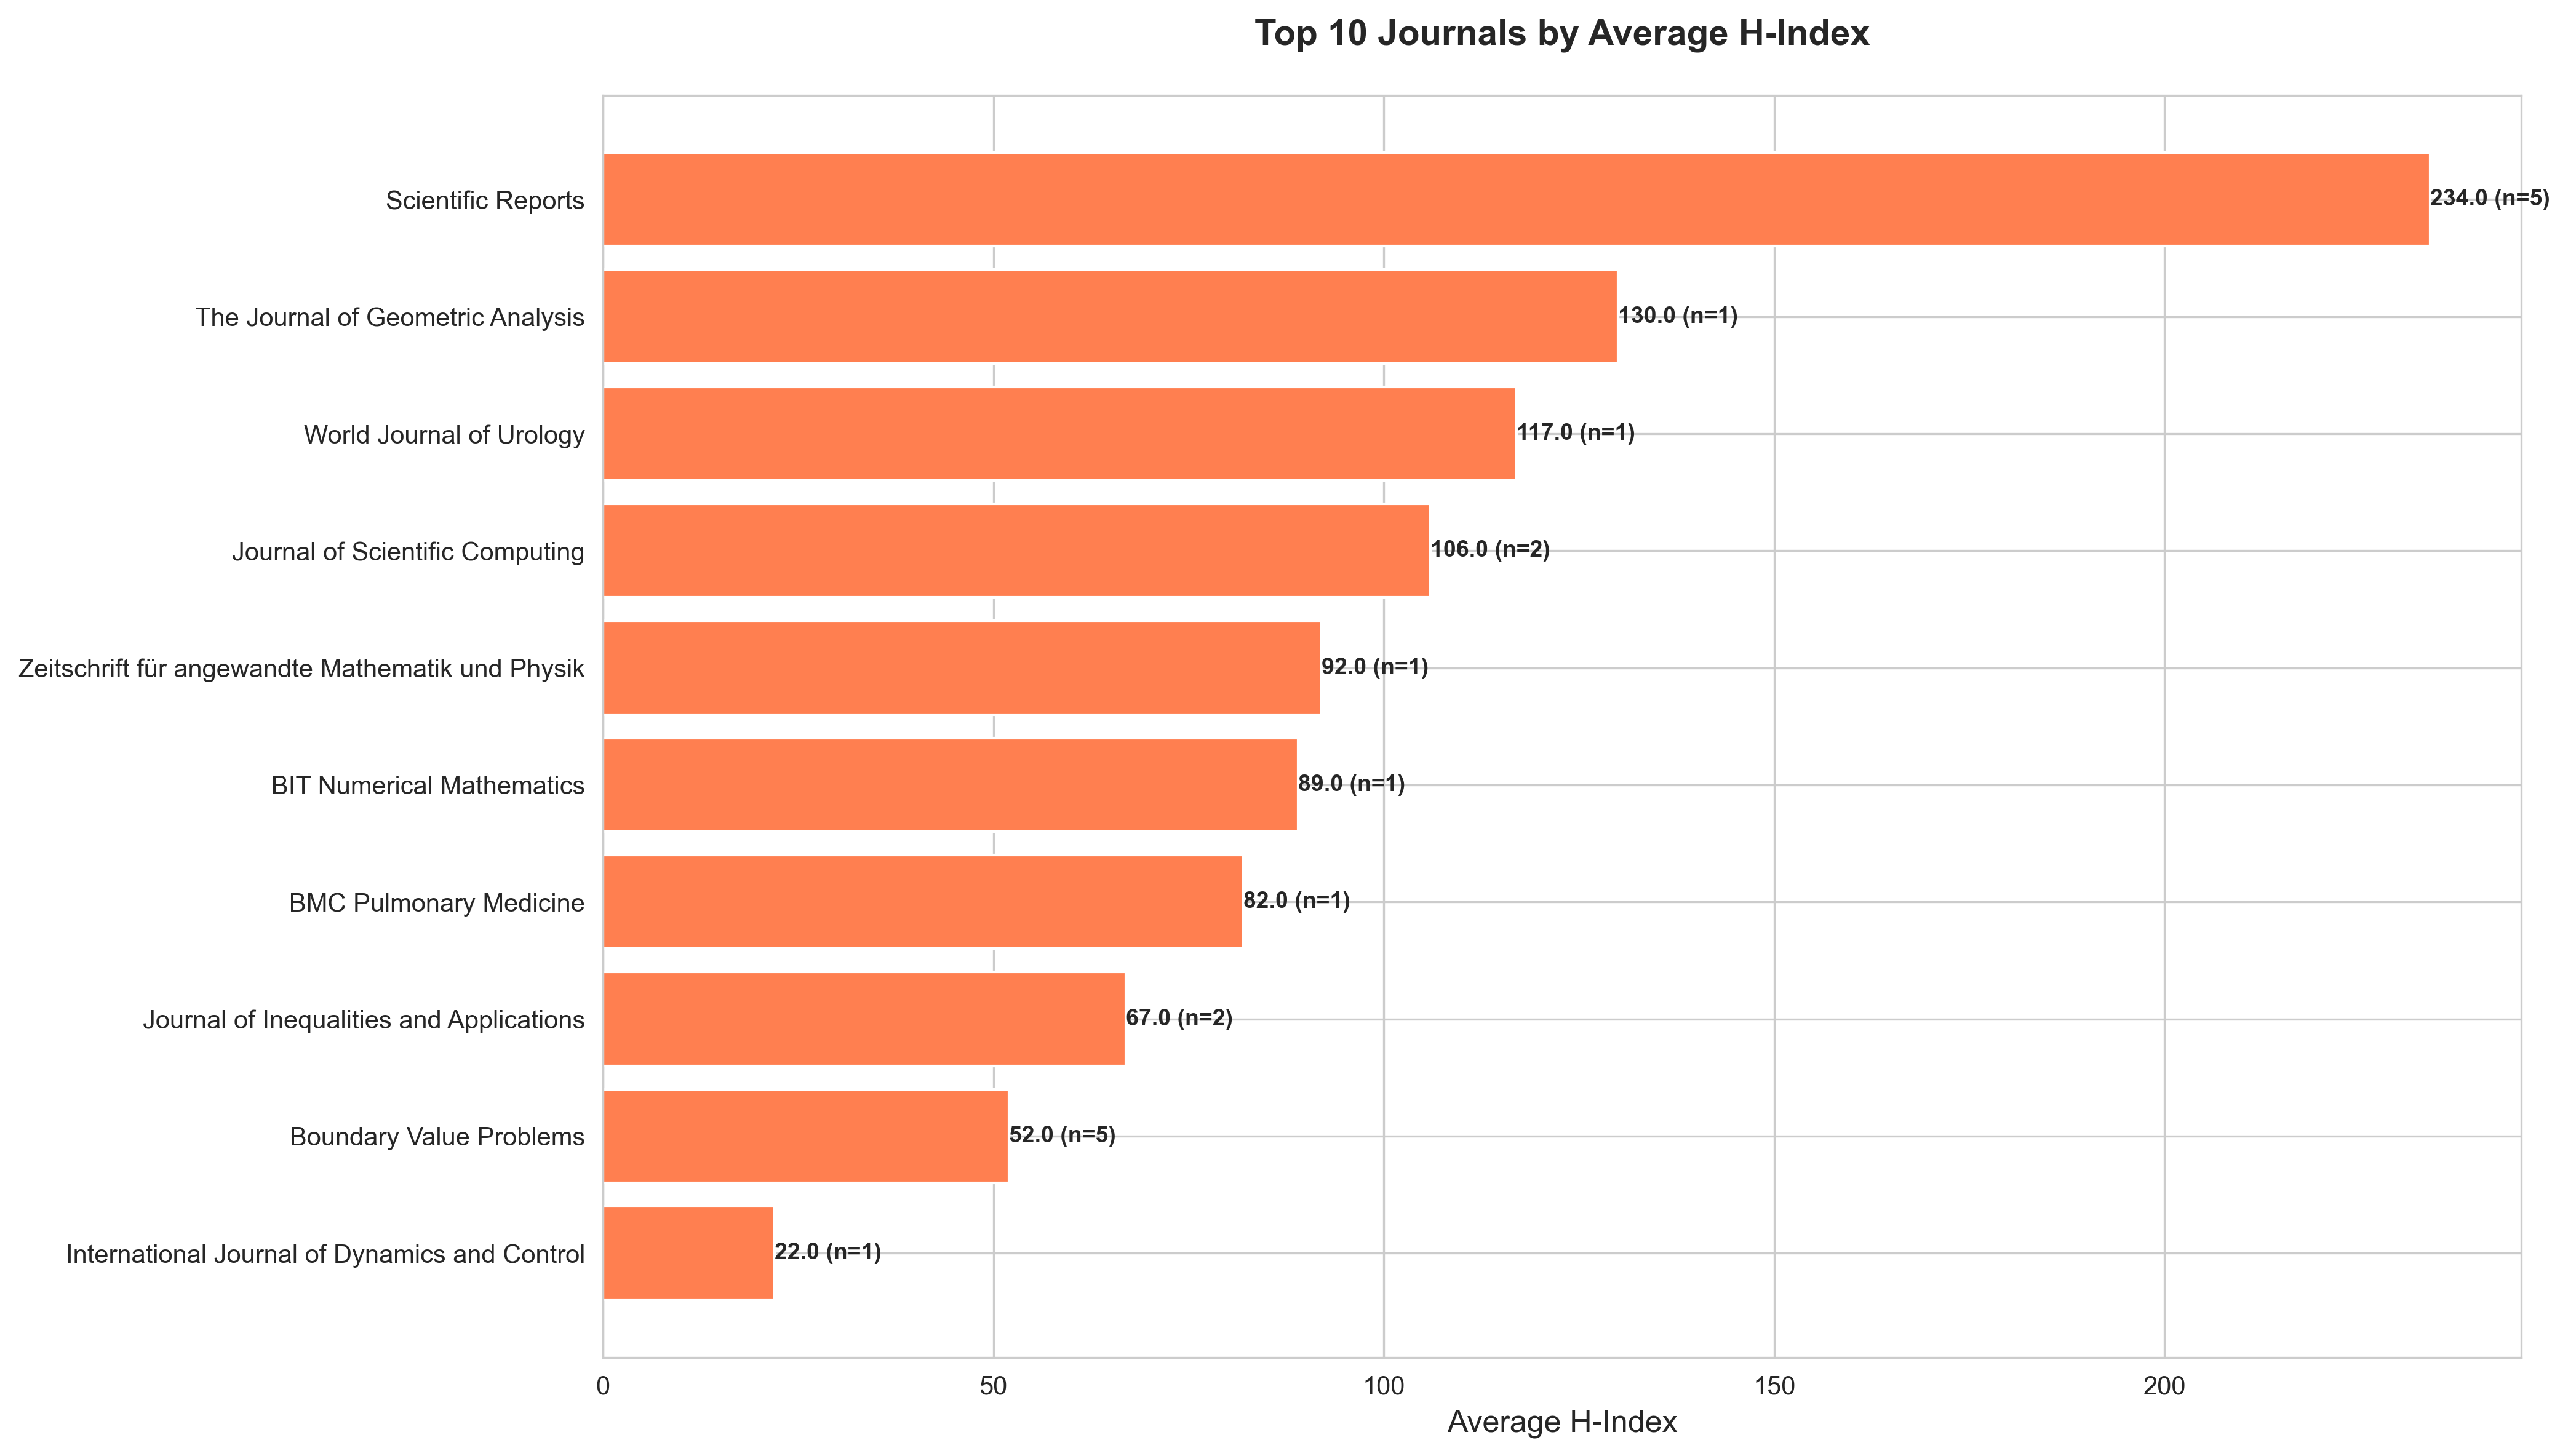
\includegraphics[width=\textwidth]{sections/Images/top_journals.png}
            \end{figure}
        \end{column}
    \end{columns}
\end{frame}

\begin{frame}{Implementation}
    \small
    \textcolor{red_unipd}{\Large Springer API Query}
    \vspace{0.5em}

    \begin{block}{Query Explanation}
        \begin{itemize}
            \item Searches for papers containing PDE-related keywords
            \item Filters only journal articles (excludes books, chapters, etc.)
            \item Restricts to publications from January 2024 to February 2026
        \end{itemize}
    \end{block}

    \begin{figure}
        \centering
        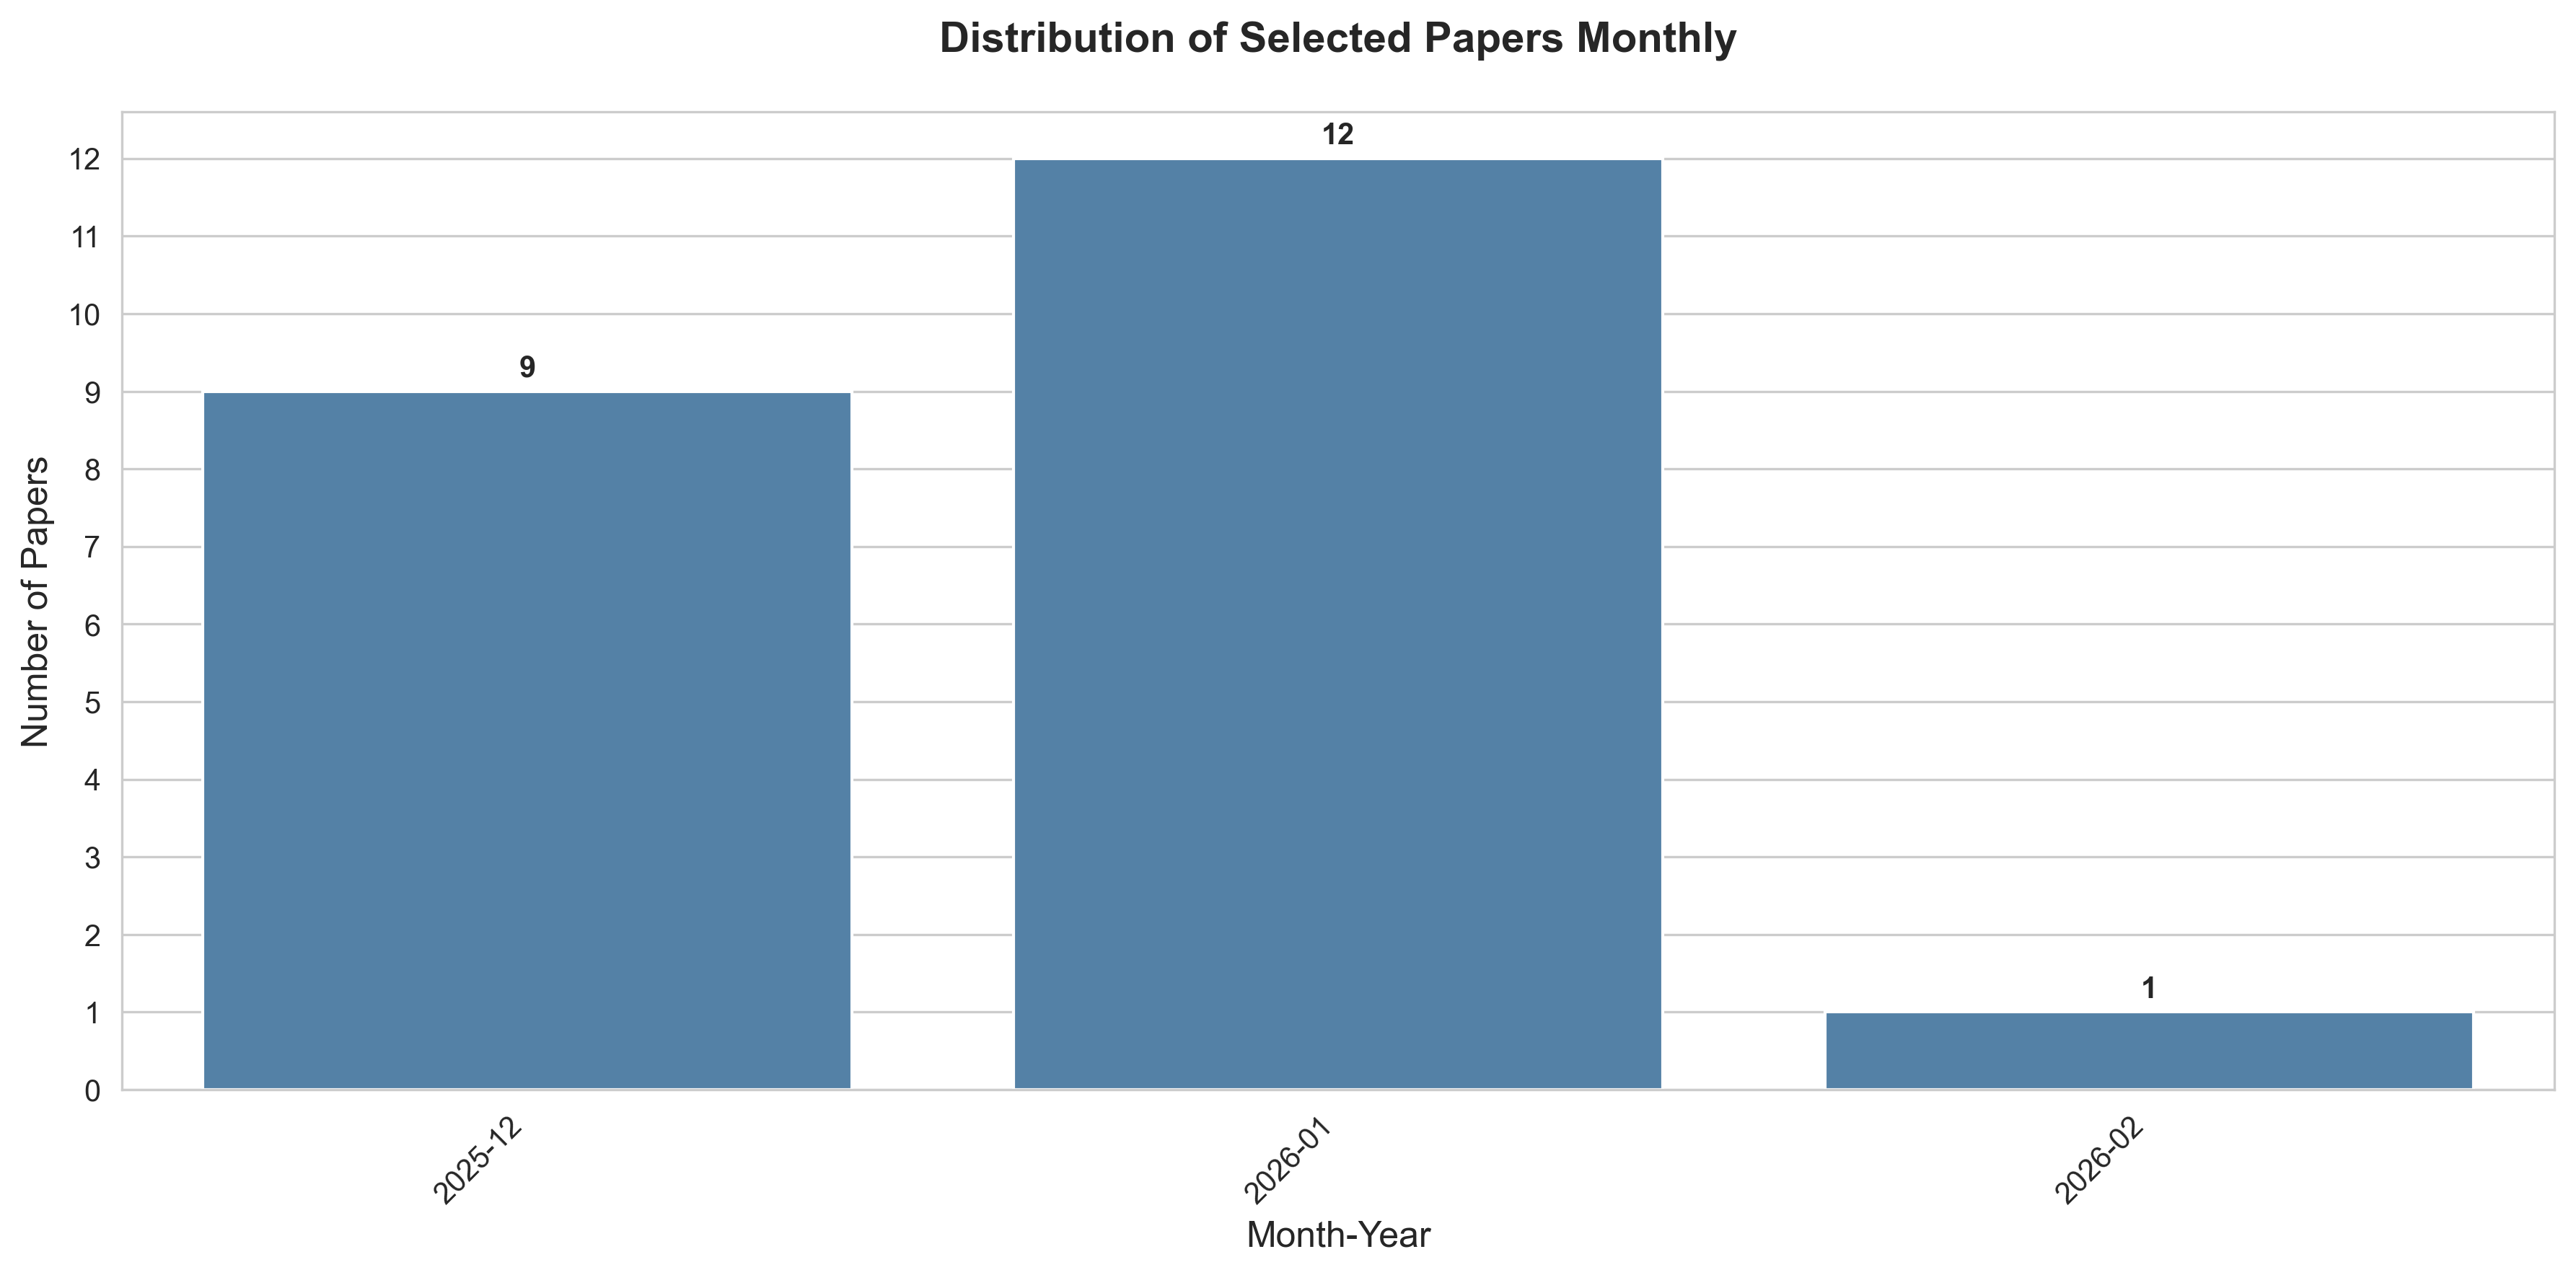
\includegraphics[width=0.7\textwidth]{sections/Images/publications_per_month.png}
    \end{figure}
\end{frame}

\begin{frame}{State of the Art}
    \small
    \textcolor{red_unipd}{\Large Numerical Methods \& Computational Mathematics 1/2}
    \vspace{0.3em}

    \centering
    \tiny
    \begin{tabular}{|c|p{3.8cm}|c|p{5cm}|}
        \hline
        \textbf{\#} & \textbf{Topic} & \textbf{H-index} & \textbf{Application} \\
        \hline
        1 & \href{http://dx.doi.org/10.1007/s10543-026-01107-x}{Hybrid Nitsche method} (02/2026) & 89 & Extends distributed FE method to arbitrary polynomial degree; simplifies transformation of FE systems to reduced basis for large-scale computing \\
        \hline
        2 & \href{http://dx.doi.org/10.1007/s10915-025-03172-w}{FourierIdent} (01/2026) & 106 & Identifies differential equations in frequency domain using Fourier analysis; reverse-engineers PDEs from observational data \\
        \hline
        3 & \href{http://dx.doi.org/10.1186/s13661-025-02202-8}{Fractional PDEs (Chebyshev)} (01/2026) & 52 & Uses second-kind Chebyshev collocation to solve nonlinear fractional diffusion, wave, and Korteweg-De Vries equations \\
        \hline
        4 & \href{http://dx.doi.org/10.1186/s13661-025-02211-7}{TLSM for fractional KdV} (01/2026) & 52 & Tantawy Least Square Method for fractional-order PDEs; achieves approximate solutions with minimal residual error \\
        \hline
        5 & \href{http://dx.doi.org/10.1007/s10915-025-03153-z}{Stochastic Ginzburg-Landau} (12/2025) & 106 & Proves convergence of numerical methods for stochastic complex Ginzburg-Landau equation with additive noise \\
        \hline
    \end{tabular}
\end{frame}

\begin{frame}{State of the Art}
    \small
    \textcolor{red_unipd}{\Large Numerical Methods \& Computational Mathematics 2/2}
    \vspace{0.3em}

    \centering
    \tiny
    \begin{tabular}{|c|p{3.8cm}|c|p{5cm}|}
        \hline
        \textbf{\#} & \textbf{Topic} & \textbf{H-index} & \textbf{Application} \\
        \hline
        6 & \href{http://dx.doi.org/10.1186/s13661-026-02226-8}{Novel integral transform} (01/2026) & 52 & Introduces novel integral transform with unique properties for more efficient solutions of linear ODEs and PDEs \\
        \hline
        7 & Parabolic completeness & N/A & Proves completeness theorems for polynomial solutions; theoretical foundations for parabolic PDE approximation \\
        \hline
        8 & \href{http://dx.doi.org/10.1007/s40435-025-01945-7}{Fractional Riesz derivative} (12/2025) & 22 & Models mass transport through polymeric membranes using time-variable space-fractional Riesz derivative; drug delivery systems \\
        \hline
        9 & \href{http://dx.doi.org/10.1007/s12220-025-02283-y}{Translators in 3D} (12/2025) & 130 & Proves geometric properties of complete translators in 3D space; geometric analysis and mean curvature flow theory \\
        \hline
    \end{tabular}
\end{frame}

\begin{frame}{State of the Art}
    \small
    \textcolor{red_unipd}{\Large Solitons \& Nonlinear Wave Phenomena}
    \vspace{0.5em}

    \centering
    \tiny
    \begin{tabular}{|c|p{4cm}|c|p{5cm}|}
        \hline
        \textbf{\#} & \textbf{Topic} & \textbf{H-index} & \textbf{Application} \\
        \hline
        1 & \href{http://dx.doi.org/10.1186/s13661-026-02233-9}{Jaulent-Miodek system} (01/2026) & 52 & Models using $\phi$-Caputo fractional derivative; captures nonlocal and memory-related effects in wave propagation using RPS and NIM methods \\
        \hline
        2 & \href{http://dx.doi.org/10.1186/s13661-025-02215-3}{Sasa-Satsuma solitons} (01/2026) & 52 & Derives soliton solutions for ultra-short pulse propagation in optical fibers; accounts for third-order dispersion, self-steepening, and stimulated scattering \\
        \hline
        3 & \href{http://dx.doi.org/10.1038/s41598-025-25497-0}{Kink solitons under noise} (12/2025) & 234 & Investigates how additive white noise affects kink solitons in power-law nonlinear Schrodinger equation; understanding soliton stability \\
        \hline
    \end{tabular}
\end{frame}

\begin{frame}{State of the Art}
    \small
    \textcolor{red_unipd}{\Large Applied Physics \& Engineering}
    \vspace{0.5em}

    \centering
    \tiny
    \begin{tabular}{|c|p{4cm}|c|p{5cm}|}
        \hline
        \textbf{\#} & \textbf{Topic} & \textbf{H-index} & \textbf{Application} \\
        \hline
        1 & \href{http://dx.doi.org/10.1038/s41598-026-35857-z}{Step-up/down converter} (01/2026) & 234 & Proposes new converter design for battery energy storage with higher power density; circuit modeling and power flow optimization using PDEs \\
        \hline
        2 & \href{http://dx.doi.org/10.1038/s41598-025-34636-6}{Bentonite-graphite spectroscopy} (01/2026) & 234 & Uses VIS-NIR spectroscopy to evaluate material homogeneity for nuclear waste repositories; diffusion and thermal conductivity modeling \\
        \hline
        3 & \href{http://dx.doi.org/10.1007/s00033-025-02651-2}{Poroelasticity homogenization} (12/2025) & 92 & Derives Biot's poroelasticity equations from microstructure using homogenization; modeling fluid flow in soil and biological tissues \\
        \hline
        4 & \href{http://dx.doi.org/10.1038/s41598-025-28168-2}{Filtration model} (12/2025) & 234 & Models contaminant transfer through water filters with chemical reactions; incorporates sorption, convection for water treatment design \\
        \hline
    \end{tabular}
\end{frame}

\begin{frame}{State of the Art}
    \small
    \textcolor{red_unipd}{\Large Other Categories}
    \vspace{0.5em}

    \centering
    \fontsize{5}{6}\selectfont
    \begin{tabular}{|c|p{1cm}|p{2.2cm}|c|p{6cm}|}
        \hline
        \textbf{\#} & \textbf{Cat.} & \textbf{Topic} & \textbf{H} & \textbf{Application} \\
        \hline
        1 & Math & \href{http://dx.doi.org/10.1186/s13660-026-03435-6}{Mulholland} (01/26) & 67 & {\fontsize{4}{5}\selectfont Derives new inequality involving partial sums;
         theoretical foundations for analysis and optimization} \\
        \hline
        2 & Stability & \href{http://dx.doi.org/10.1186/s13660-025-03404-5}{Frac. damping} (01/26) & 67 & {\fontsize{4}{5}\selectfont Analyzes wave equation stabilization with varying fractional damping; semigroup theory for energy decay} \\
        \hline
        3 & Neuro & \href{http://dx.doi.org/10.1038/s41598-025-32388-x}{Brain connect.} (12/25) & 234 & {\fontsize{4}{5}\selectfont Studies intracortical and corticomuscular connectivity during reach-and-grasp movements using PDC analysis} \\
        \hline
        4 & Neuro & \href{http://dx.doi.org/10.1186/s40708-025-00283-w}{PDE fMRI} (12/25) & 16 & {\fontsize{4}{5}\selectfont Applies PDE modeling to fMRI data using SINDy and PDE-Net 2.0; identifies underlying brain dynamics} \\
        \hline
        5 & Ecology & Leslie-Gower & N/A & {\fontsize{4}{5}\selectfont Studies predator-prey dynamics with fear effects and spatial diffusion; reaction-diffusion equations} \\
        \hline
    \end{tabular}
\end{frame} % Lucia
\section{Mathematical Background}


% ===== Slide 1 (Navier–Stokes) =====
\begin{secframe}
\small
\textcolor{red_unipd}{\Large General Form of Navier--Stokes Equations}

\vspace{0.6em}

\begin{alertblock}{Equations}
\[
\begin{cases}
\dfrac{\partial \rho}{\partial t}
+ \nabla\!\cdot\!(\rho \mathbf{u}) = 0,\\[16pt]

\dfrac{\partial (\rho \mathbf{u})}{\partial t}
+ \nabla\!\cdot\!(\rho \mathbf{u} \otimes \mathbf{u})
= -\nabla p + \nabla\!\cdot\!\boldsymbol{\Sigma} + \rho \mathbf{g},\\[16pt]

\dfrac{\partial E}{\partial t}
+ \nabla\!\cdot\!((E+p)\mathbf{u})
= \nabla\!\cdot\!(\boldsymbol{\tau}\!\cdot\!\mathbf{u})
- \nabla\!\cdot\!\mathbf{q} + \rho \mathbf{u}\!\cdot\!\mathbf{g}
\end{cases}
\]
\end{alertblock}

\end{secframe}




% ===== New Slide 3: Physical Meaning -- Mass Conservation =====
\begin{secframe}
\small
\textcolor{red_unipd}{\Large Conservation Laws: Mass}

\vspace{0.8em}

\begin{alertblock}{Continuity equation -- Mass Conservation}
\[
\dfrac{\partial \rho}{\partial t} + \nabla\!\cdot\!(\rho \mathbf{u}) = 0
\]
\end{alertblock}

\begin{block}{Term definitions}
\begin{itemize}
  \item \(\rho\): fluid density \([\text{kg·m}^{-3}]\)
  \item \(\mathbf{u} = (u,v,w)\): velocity field \([\text{m·s}^{-1}]\)
  \item \(\nabla\!\cdot\!(\rho \mathbf{u})\): divergence of mass flux
  \item \(\partial \rho / \partial t\): local time rate of change of density
\end{itemize}
\end{block}
\end{secframe}




% ===== Slide 4: Physical Meaning -- Momentum Conservation =====
\begin{secframe}
\small
\textcolor{red_unipd}{\Large Conservation Laws: Momentum}

\vspace{0.8em}

\begin{alertblock}{Newton’s second law -- Momentum equation}
\[
\dfrac{\partial (\rho \mathbf{u})}{\partial t}
+ \nabla\!\cdot\!(\rho \mathbf{u}\otimes\mathbf{u})
= -\nabla p + \nabla\!\cdot\!\boldsymbol{\Sigma} + \rho \mathbf{g}
\]
\end{alertblock}

\begin{block}{Term definitions}
\begin{itemize}
  \item \(\rho \mathbf{u}\): momentum density \([\text{kg·m}^{-2}\text{·s}^{-1}]\)
  \item \(\nabla\!\cdot\!(\rho \mathbf{u}\otimes\mathbf{u})\): convective momentum transport
  \item \(-\nabla p\): pressure gradient force per unit volume
  \item \(\boldsymbol{\Sigma}\): viscous stress tensor \([\text{Pa}]\)
  \item \(\rho \mathbf{g}\): body force density (e.g. gravity) \([\text{N·m}^{-3}]\)
\end{itemize}
\end{block}
\end{secframe}




% ===== Slide 5: Physical Meaning -- Energy Conservation =====
\begin{secframe}
\small
\textcolor{red_unipd}{\Large Conservation Laws: Energy}

\vspace{0.8em}

\begin{alertblock}{Energy equation (first law of thermodynamics)}
\[
\dfrac{\partial E}{\partial t}
+ \nabla\!\cdot\!((E+p)\mathbf{u})
= \nabla\!\cdot\!(\boldsymbol{\tau}\!\cdot\!\mathbf{u})
- \nabla\!\cdot\!\mathbf{q}
+ \rho \mathbf{u}\!\cdot\!\mathbf{g}
\]
\end{alertblock}

\begin{block}{Term definitions}
\begin{itemize}
  \item \(E = \rho\!\left(e + \tfrac{1}{2}|\mathbf{u}|^2\right)\): total energy density (internal + kinetic)
  \item \(p\): pressure \([\text{Pa}]\)
  \item \(\boldsymbol{\tau}\): stress tensor (viscous + pressure)
  \item \(\mathbf{q}\): heat flux vector \([\text{W·m}^{-2}]\)
  \item \(\rho \mathbf{u}\!\cdot\!\mathbf{g}\): work done by body forces
\end{itemize}
\end{block}
\end{secframe}




% ===== Slide 6 =====
\begin{secframe}
\small
\textcolor{red_unipd}{\Large Newtonian Hypotheses and Constitutive Relations}

\begin{alertblock}{Viscous Stress}
\[
\begin{cases}
\boldsymbol{\Sigma} = \mu\left(\nabla \mathbf{u} + (\nabla \mathbf{u})^T\right) + \lambda (\nabla\!\cdot\!\mathbf{u}) \mathbf{I},\\[4pt]
\boldsymbol{\tau} = \boldsymbol{\Sigma} - p \mathbf{I}
\end{cases}
\]
\end{alertblock}

\begin{alertblock}{Heat Flux}
\[
\mathbf{q} = -k \nabla T
\]
\end{alertblock}

\begin{alertblock}{Internal Energy}
\[
E = \rho\left(e + \dfrac{1}{2}|\mathbf{u}|^2\right)
\]
\end{alertblock}

\end{secframe}




% ===== Slide 7 (Navier–Stokes with Constitutive Relations Expanded) =====
\begin{secframe}
\small
\textcolor{red_unipd}{\Large General Form with Constitutive Relations Expanded}

\vspace{0.6em}

\begin{alertblock}{Equations (Newtonian, compressible, viscous fluid)}
\[
\begin{cases}
\dfrac{\partial \rho}{\partial t}
+ \nabla\!\cdot\!(\rho \mathbf{u}) = 0,\\[16pt]

\rho\!\left(
\dfrac{\partial \mathbf{u}}{\partial t}
+ (\mathbf{u}\!\cdot\!\nabla)\mathbf{u}
\right)
= -\nabla p
+ \nabla\!\cdot\!\Big[
\mu\!\left(\nabla \mathbf{u} + (\nabla \mathbf{u})^T\right)
+ \lambda (\nabla\!\cdot\!\mathbf{u})\mathbf{I}
\Big]
+ \rho \mathbf{g},\\[20pt]

\dfrac{\partial }{\partial t}\!
\left[\rho\!\left(e + \dfrac{1}{2}|\mathbf{u}|^2\right)\right]
+ \nabla\!\cdot\!
\left[\rho\!\left(e + \dfrac{1}{2}|\mathbf{u}|^2\right)\mathbf{u} + p\mathbf{u}\right]
= \\ \nabla\!\cdot\!
\Big\{
\mu\!\left(\nabla \mathbf{u} + (\nabla \mathbf{u})^T\right)\!\cdot\!\mathbf{u}
+ \lambda (\nabla\!\cdot\!\mathbf{u})\mathbf{u}
- k\nabla T
\Big\}
+ \rho \mathbf{u}\!\cdot\!\mathbf{g}
\end{cases}
\]
\end{alertblock}

\end{secframe}




% ===== Slide 8 =====
\begin{secframe}
\small
\textcolor{red_unipd}{\Large Why Navier--Stokes Matters in Neural PDEs}

\vspace{0.6em}

\begin{block}{Central role in neural modeling}
The Navier--Stokes system unifies diffusion (viscous term),  
advection (nonlinear term), and incompressibility (constraint).  
Each paper tests neural architectures by simplifying or approximating parts of this system:
\begin{itemize}
  \item \textbf{PINNs:} direct enforcement of differential operators;
  \item \textbf{FNOs:} operator learning across time steps of Navier–Stokes;
  \item \textbf{NFTM:} learned iterative refinement mimicking PDE rollouts.
\end{itemize}
\vspace{0.4em}
Through these methods, the goal is to determine whether deep neural architectures can reproduce  
\textit{the stability and accuracy of physical solvers} for complex spatio-temporal dynamics.
\end{block}
\end{secframe}






% ===== Slide 1 =====
\begin{secframe}
\small
\textcolor{red_unipd}{\Large Burgers Equation as a Simplified Model}

\vspace{0.6em}

\begin{alertblock}{Equation}
\[
\begin{cases}
  u_t + u u_x + v u_y = \nu (u_{xx} + u_{yy}), \\
  v_t + u v_x + v v_y = \nu (v_{xx} + v_{yy})
\end{cases}
\]
\end{alertblock}

\vfill

\begin{block}{Hypotheses}
\(\nabla p=\mathbf{0}\). \quad
1D reduction: \(\mathbf{u}=(u(x,t),0)\). \quad
Self-advection: \(u\,\partial_x u\).
\end{block}

\vspace{0.5em}

\begin{block}{Einstein notation}
$u_t = \frac{\partial u}{\partial t}$, $u_x = \frac{\partial u}{\partial x}$, $u_{xx} = \frac{\partial^2 u}{\partial x^2}$, etc.
\end{block}

\end{secframe}

% ===== Advection Frame =====
\begin{secframe}
\small
\textcolor{red_unipd}{\Large Advection}

\vspace{0.6em}

\begin{block}{Advection Terms}
\begin{itemize}
    \item \textbf{$u u_x$, $v v_y$, $u v_x$, $v u_y$}: Nonlinear advection terms.
    \item Represent transport of velocity due to the flow itself.
\end{itemize}
\end{block}

\begin{figure}[h]
    \centering
    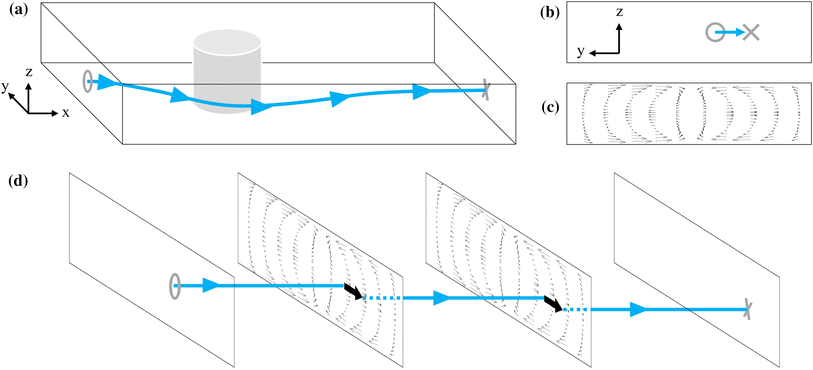
\includegraphics[width=0.7\linewidth]{images/theory/advection.png}
\end{figure}

\end{frame}

% ===== Diffusion Frame =====
\begin{frame}{2D Burgers Equation}
\small
\textcolor{red_unipd}{\Large Diffusion}

\vspace{0.6em}

\begin{block}{Diffusion Terms}
\begin{itemize}
    \item \textbf{$\nu (u_{xx} + u_{yy})$, $\nu (v_{xx} + v_{yy})$}: Diffusion terms.
    \item Model the spreading and smoothing of velocity due to viscosity $\nu$.
\end{itemize}
\end{block}

\begin{figure}[h]
    \centering
    
\includegraphics[width=0.7\linewidth]{images/theory/diffusion.png}
\end{figure}


\end{secframe}

% ===== Balance Frame =====
\begin{secframe}
\small
\textcolor{red_unipd}{\Large Pressure gradient}

\vspace{0.6em}

\begin{alertblock}{Pressure Gradient Terms}
  The huge Hypotheses here is \(\nabla p=\mathbf{0}\), so there is no effect of the pressure in the equation. \\
  \( \Rightarrow \) Only the initial velocity has an influence on the evolution of the system
\end{alertblock}

\begin{example}
  Consider a scenario where the initial velocity is constant across the domain on airfoil shape. \\
  Since \(\nabla p=\mathbf{0}\), the pressure gradient does not influence the flow. \\
  The flow will not change over time, remaining constant as per the initial condition.
\end{example}



\end{secframe}

% ===== Slide 2 =====
\begin{secframe}
\small
\textcolor{red_unipd}{\Large Numerical Simulation}

\vspace{0.6em}

\begin{block}{Description}
\begin{itemize}
  \item Implements the PDE directly using finite difference methods.
  \item Discretizes space and time; updates velocity fields step by step.
  \item Parameters: grid size, time step, viscosity, initial/boundary conditions.
\end{itemize}
\end{block}

\begin{alertblock}{Finite Difference Schemes}
\begin{itemize}
  \item Forward difference (time): $u_t \approx \frac{u_{i,j}^{n+1} - u_{i,j}^n}{\Delta t}$
  \item Central difference (space): $u_x \approx \frac{u_{i+1,j}^n - u_{i-1,j}^n}{2\Delta x}$
  \item Central difference (second derivative): $u_{xx} \approx \frac{u_{i+1,j}^n - 2u_{i,j}^n + u_{i-1,j}^n}{\Delta x^2}$
\end{itemize}
\end{alertblock}

\end{secframe}




\section{2D Neural Model}

% ===== Slide 1: Overview =====
\begin{secframe}
\small
\textcolor{red_unipd}{\Large 2D Neural Network Pipeline}

\vspace{0.6em}

\begin{block}{Goal}
Learn to predict 2D Burgers trajectories $\mathbf{u}(x,y,t)$ from short histories.
\end{block}

\begin{block}{Pipeline}
\begin{itemize}
  \item Load generated 2D dataset (train/test) with viscosity labels $\nu$.
  \item Train a Transformer-based controller on sequences of frames.
  \item Evaluate: trajectory rollout and error over time.
\end{itemize}
\end{block}

\end{secframe}



% % ===== Slide 2: Dataset =====
% \begin{secframe}
% \small
% \textcolor{red_unipd}{\Large 2D Dataset Configuration}

% \vspace{0.6em}

% \begin{block}{Source}
% Generated 2D Burgers dataset with separate train/test folders.
% \end{block}

% \begin{block}{Key settings}
% \begin{itemize}
%   \item Dataset type: generated 2D samples.
%   \item History length: $3$ frames.
%   \item Batch size: $4$.
%   \item Input grid inferred from data: $(C, H, W)$.
% \end{itemize}
% \end{block}

% \end{secframe}



% % ===== Slide 3: Model =====
% \begin{secframe}
% \small
% \textcolor{red_unipd}{\Large 2D Transformer Controller}

% \vspace{0.6em}

% \begin{block}{Architecture}
% TransformerController2D with patch-based tokens.
% \end{block}

% \begin{block}{Hyperparameters}
% \begin{itemize}
%   \item Patch radius: $r=0$ \;\; ($\text{patch size} = C(2r+1)^2$).
%   \item Hidden size: $64$.
%   \item Output channels: $C$.
%   \item Chunk size: $5$ (sequential rollout).
% \end{itemize}
% \end{block}

% \end{secframe}



% % ===== Slide 4: Training =====
% \begin{secframe}
% \small
% \textcolor{red_unipd}{\Large Training Setup}

% \vspace{0.6em}

% \begin{block}{Training loop}
% \begin{itemize}
%   \item $40$ epochs of supervised learning.
%   \item Loss tracked over epochs and visualized after training.
%   \item Optional model loading/saving for checkpoints.
% \end{itemize}
% \end{block}

% \begin{alertblock}{Objective}
% Minimize trajectory prediction error over time for the chosen $\nu$.
% \end{alertblock}

% \end{secframe}



% % ===== Slide 5: Evaluation =====
% \begin{secframe}
% \small
% \textcolor{red_unipd}{\Large Evaluation and Visualization}

% \vspace{0.6em}

% \begin{block}{Evaluation}
% \begin{itemize}
%   \item Select a target viscosity $\nu$ (fixed or random).
%   \item Rollout prediction vs. ground truth on test data.
%   \item Compute relative $\ell_2$ error over time.
% \end{itemize}
% \end{block}

% \begin{block}{Outputs}
% \begin{itemize}
%   \item Animated 2D fields (true, predicted, error).
%   \item Error curve summarizing stability across time.
% \end{itemize}
% \end{block}

% \end{secframe} % Samuel
% \input{sections/NS-Simplified.tex}
% \input{sections/1D Burgers Equation.tex} % Samuel
% \input{sections/2D Burgers Equation.tex}
\section{Project Pipeline}

\begin{secframe}
    Project pipeline
\end{secframe} % Alex
\section{1D Burgers Equation Dataset}

%% ---------------------------------------------------------------
%% SLIDE 1: Dataset structure
%% ---------------------------------------------------------------
\begin{frame}{\large Dataset: 1D Burgers Equation Trajectories}
\vspace{-0.5em}
  \begin{columns}[t]
    \begin{column}{0.55\textwidth}
      \begin{block}{\centering \small Where does the data come from?}
        We use the \textbf{official dataset} from the FNO paper
        (Li et al., 2021). The trajectories were generated by
        numerically solving the 1D Burgers equation and saving
        the full solution over time.
        \begin{itemize}\setlength\itemsep{1pt}
          \item \textbf{Domain}: $x \in [0,1]$, $t \in [0,1]$.
          \item \textbf{Periodic boundary conditions}.
          \item Fixed \textbf{viscosity} values: $\nu \in \{0.001, 0.004, 0.01, 0.02, 0.1, 0.3, 0.5, 0.7\}$.
          \item \textbf{1000 train + 200 test} per resolution.
        \end{itemize}
      \end{block}
    \end{column}
    \begin{column}{0.46\textwidth}
      \begin{block}{\centering \small Four grid resolutions}
        \begin{center}
        \small {$85 \times 85$, $141 \times 141$,}\\[0.4em] \small{$211 \times 211$, $421 \times 421$}
        \end{center}
      \end{block}
      \begin{block}{\centering \small Initial conditions}
        \begin{itemize}
            \item The initial condition $u(x,0)$ is randomly generated for each trajectory.
            \item \item From three families:
            \begin{itemize}\setlength\itemsep{1pt}
              \item \textbf{Random Fourier modes:} $u(x,0) = \sum_{n=1}^N A_n \sin(2\pi k_n x + \phi_n)$, with random $A_n$, $k_n$, and $\phi_n$.
              \item \textbf{Single sine waves:} $u(x,0) = A \sin(2\pi k x + \phi)$, with random $A$, $k$, and $\phi$.
              \item \textbf{Two-mode sines:} $u(x,0) = A_1 \sin(2\pi k_1 x + \phi_1) + A_2 \sin(2\pi k_2 x + \phi_2)$, with random parameters.
            \end{itemize}
            \item This variety ensures the model learns to handle a wide range of initial conditions, from simple to complex.
        \end{itemize}
        \end{block}
    \end{column}
  \end{columns}

\end{frame}

%% ---------------------------------------------------------------
%% SLIDE 2: Visualizations - 2x2 grid (s=85 and s=421, nu=0.01 and nu=0.3)
%% Replace each \fbox with \includegraphics[width=\linewidth]{path/to/image.png}
%% ---------------------------------------------------------------
\begin{frame}{Visualizing the Data: 2x2 Grid of Trajectories}

  % Column headers
  \begin{columns}[c]
    \begin{column}{0.02\textwidth}\end{column}
    \begin{column}{0.47\textwidth}
      \centering\small\textbf{$\nu = 0.01$ --- shock}
    \end{column}
    \begin{column}{0.47\textwidth}
      \centering\small\textbf{$\nu = 0.3$ --- smooth}
    \end{column}
  \end{columns}

  \vspace{0.2em}

  % Row 1: s=85
  \begin{columns}[c]
    \begin{column}{0.04\textwidth}
      \rotatebox{90}{\scriptsize\textbf{$s=85$}}
    \end{column}
    \begin{column}{0.46\textwidth}
      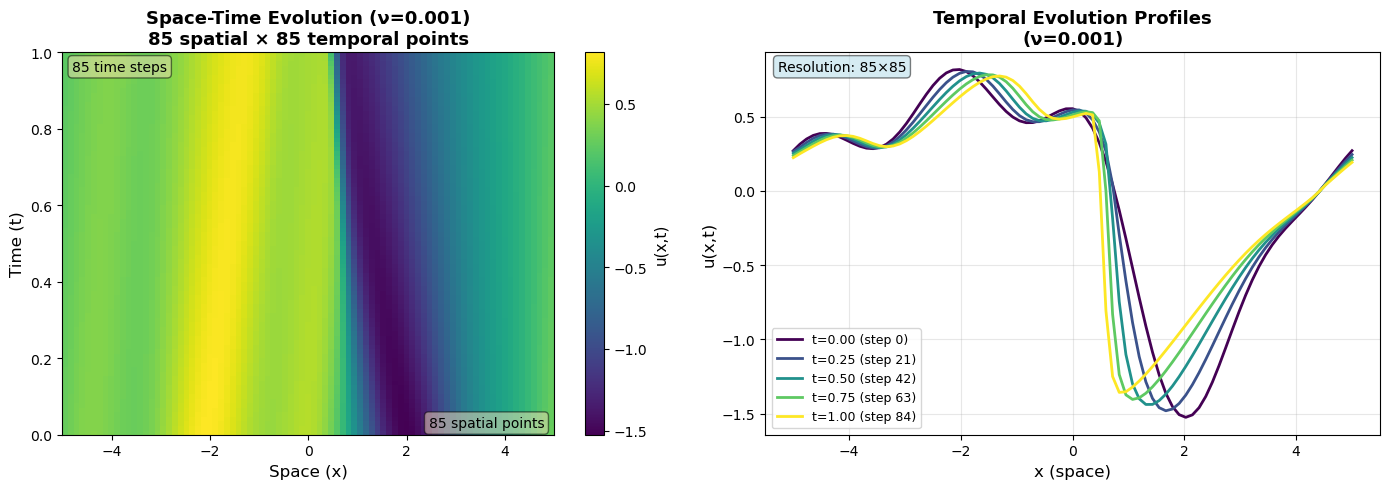
\includegraphics[width=\linewidth, height=2.5cm, keepaspectratio]
        {images/burger/sample_85x85_nu0001.png}
    \end{column}
    \begin{column}{0.46\textwidth}
      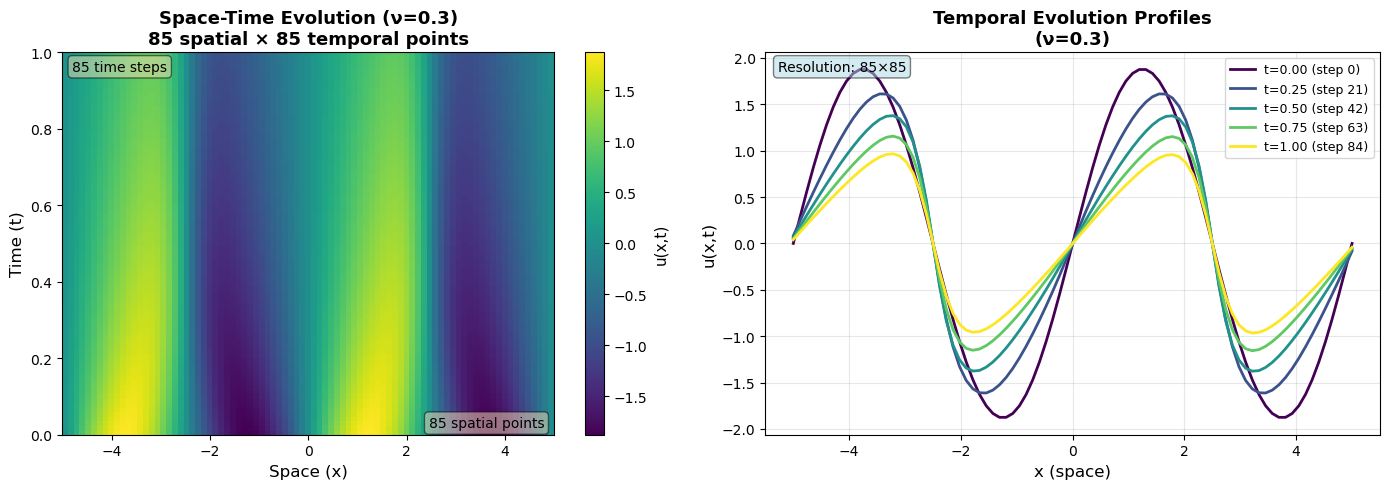
\includegraphics[width=\linewidth, height=2.5cm, keepaspectratio]
        {images/burger/sample_85x85_nu03.png}
    \end{column}
  \end{columns}

  \vspace{0.2em}

  % Row 2: s=421
  \begin{columns}[c]
    \begin{column}{0.04\textwidth}
      \rotatebox{90}{\scriptsize\textbf{$s=421$}}
    \end{column}
    \begin{column}{0.46\textwidth}
      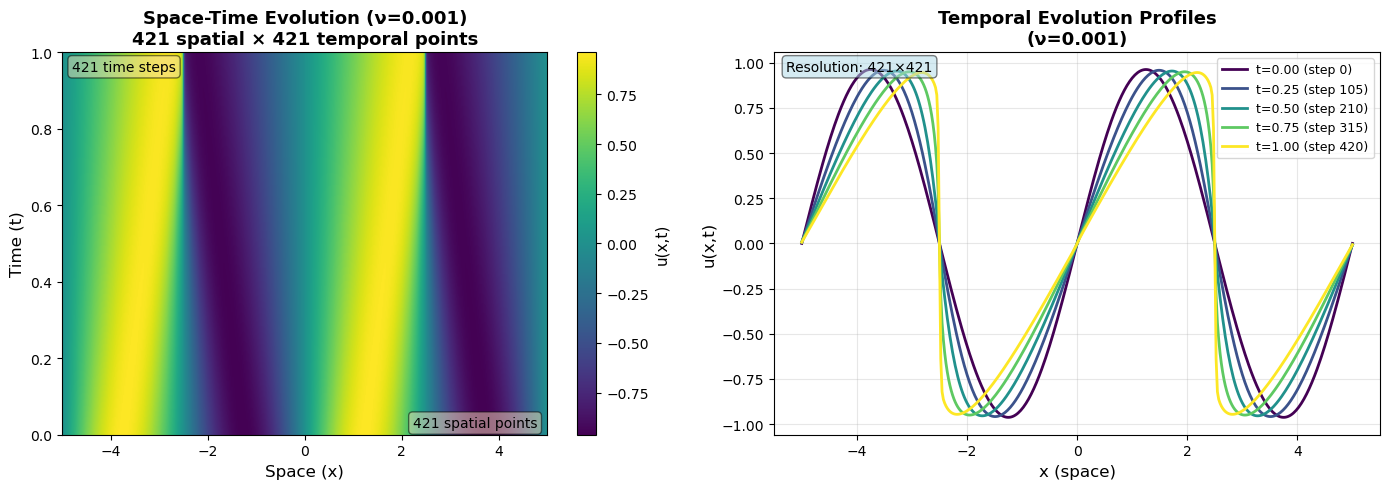
\includegraphics[width=\linewidth, height=2.5cm, keepaspectratio]
        {images/burger/sample_421x421_nu0001.png}
    \end{column}
    \begin{column}{0.46\textwidth}
      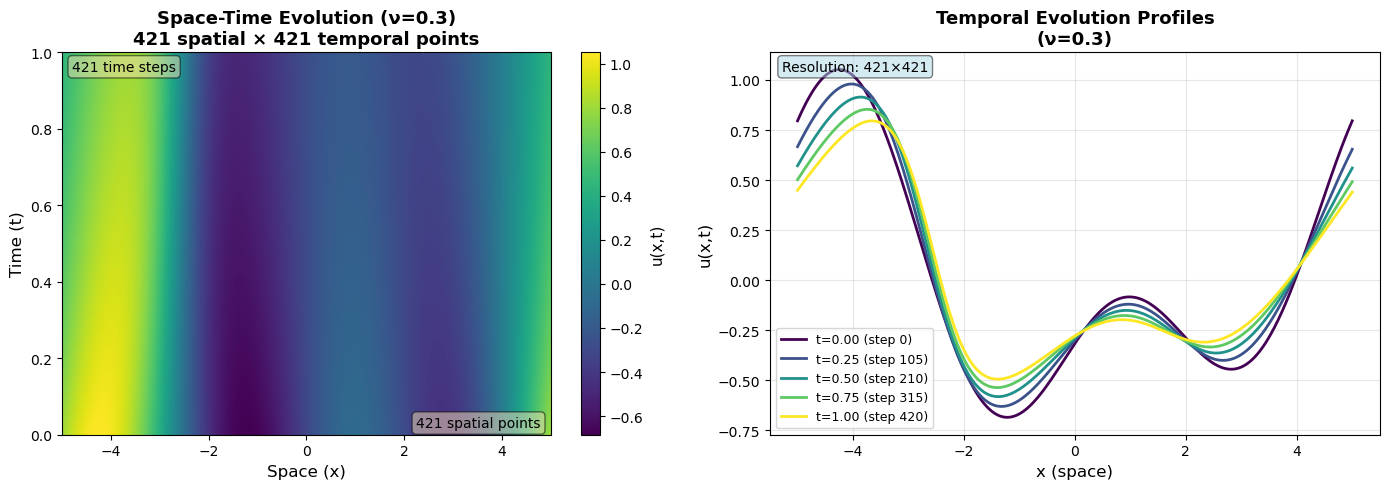
\includegraphics[width=\linewidth, height=2.5cm, keepaspectratio]
        {images/burger/sample_421x421_nu03.png}
    \end{column}
  \end{columns}

  \vspace{0.3em}

  \begin{columns}[t]
    \begin{column}{0.48\textwidth}
      \small Sharp diagonal band = shock moving across the domain.
      Finer grid ($s=421$) captures it more precisely.
    \end{column}
    \begin{column}{0.48\textwidth}
      \small Smooth gradient = diffusion spreading the wave.
      Looks similar at both resolutions --- easy case.
    \end{column}
  \end{columns}

\end{frame}

%% ---------------------------------------------------------------
%% SLIDE 3: Effect of viscosity explained
%% ---------------------------------------------------------------
\begin{frame}{Effect of Viscosity $\nu$}

  \begin{columns}[t]
    \begin{column}{0.48\textwidth}
      \begin{block}{$\nu = 0.01$ --- shock regime}
        \begin{itemize}\setlength\itemsep{2pt}
          \item Advection wins over diffusion
          \item The wave steepens and forms a \textbf{near-shock}
          \item Very sensitive to the initial condition
          \item \textbf{Hard for the model} --- fast changes, sharp features
        \end{itemize}
      \end{block}
    \end{column}
    \begin{column}{0.48\textwidth}
      \begin{block}{$\nu = 0.3$ --- smooth regime}
        \begin{itemize}\setlength\itemsep{2pt}
          \item Diffusion wins over advection
          \item The wave spreads out and flattens
          \item Predictable, regular dynamics
          \item \textbf{Easier for the model} --- slow, smooth changes
        \end{itemize}
      \end{block}
    \end{column}
  \end{columns}

  \vspace{0.4em}

  \begin{center}
  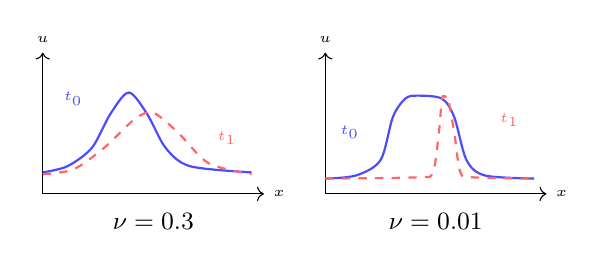
\begin{tikzpicture}[scale=0.78]
    \draw[->] (0,0)--(3.6,0) node[right]{\tiny $x$};
    \draw[->] (0,0)--(0,2.3) node[above]{\tiny $u$};
    \node at (1.8,-0.45) {\small $\nu=0.3$};
    \draw[blue!70, thick] plot[smooth] coordinates {
      (0,0.35)(0.4,0.45)(0.8,0.75)(1.1,1.3)(1.4,1.65)(1.7,1.3)(2.0,0.75)(2.4,0.45)(3.4,0.35)};
    \draw[red!60, dashed, thick] plot[smooth] coordinates {
      (0,0.32)(0.5,0.40)(1.0,0.75)(1.5,1.22)(1.8,1.32)(2.2,1.0)(2.7,0.50)(3.4,0.32)};
    \node[blue!70, font=\tiny] at (0.5,1.55) {$t_0$};
    \node[red!60,  font=\tiny] at (3.0,0.90) {$t_1$};
    \begin{scope}[xshift=4.6cm]
      \draw[->] (0,0)--(3.6,0) node[right]{\tiny $x$};
      \draw[->] (0,0)--(0,2.3) node[above]{\tiny $u$};
      \node at (1.8,-0.45) {\small $\nu=0.01$};
      \draw[blue!70, thick] plot[smooth] coordinates {
        (0,0.25)(0.5,0.30)(0.9,0.55)(1.1,1.25)(1.3,1.55)(1.5,1.60)(1.9,1.55)(2.1,1.25)(2.3,0.55)(2.6,0.30)(3.4,0.25)};
      \draw[red!60, dashed, thick] plot[smooth] coordinates {
        (0,0.25)(1.5,0.27)(1.75,0.35)(1.85,1.0)(1.90,1.55)(1.95,1.58)(2.0,1.55)(2.1,1.0)(2.2,0.35)(2.4,0.27)(3.4,0.25)};
      \node[blue!70, font=\tiny] at (0.4,1.0) {$t_0$};
      \node[red!60,  font=\tiny] at (3.0,1.2) {$t_1$};
    \end{scope}
  \end{tikzpicture}
  \end{center}

\end{frame}

%% ---------------------------------------------------------------
%% SLIDE 4: Multi-resolution evaluation
%% ---------------------------------------------------------------
\begin{frame}{Testing at 4 Different Resolutions}

  \begin{block}{Why do we test at 4 resolutions?}
    We want to know if our model works well regardless of how fine the
    grid is. A good model should give similar accuracy at $s=85$ and
    at $s=421$ --- this is called \textbf{resolution consistency}.
    We trained one TCAN model per resolution, all with the same
    architecture, and compared the results.
  \end{block}

  \vspace{0.4em}

  \begin{columns}[t]
    \begin{column}{0.48\textwidth}
      \begin{block}{What changes with resolution?}
        \begin{itemize}\setlength\itemsep{2pt}
          \item Finer grid $\Rightarrow$ more spatial points
          \item More time steps $\Rightarrow$ longer rollout
          \item Longer rollout $\Rightarrow$ more accumulated error
          \item So higher $s$ is naturally harder for TCAN
        \end{itemize}
      \end{block}
    \end{column}
    \begin{column}{0.48\textwidth}
      \begin{block}{Viscosity regimes in the data}
        \begin{center}
        \small
        \begin{tabular}{ll}
          \toprule
          $\nu$ range & Behaviour \\
          \midrule
          $(0,\,0.05)$   & Near-shock \\
          $(0.05,\,0.3)$ & Transitional \\
          $(0.3,\,1.0)$  & Smooth \\
          \bottomrule
        \end{tabular}
        \end{center}
        Since $\nu \sim \mathcal{U}(0,1)$, all three regimes
        appear in both train and test sets.
      \end{block}
    \end{column}
  \end{columns}

\end{frame} % Alex
\section{Different Approaches}


\begin{frame}{CNN/Transformer Controller Approach}
\begin{columns}[T]

\column{0.35\textwidth}
\begin{block}{Key Points}
\begin{itemize}
    \item Training and rollout loop for patch-based controllers (Transformer/RNN/CNN). Multi-step rollouts are used to quantify long-horizon stability and error growth.
\end{itemize}
\end{block}

\column{0.62\textwidth}
\begin{center}
    % Figure 4.2 from report (page 16) — General training and rollout loop
    
\includegraphics[width=\textwidth]{{images/different approaches/cnn_architecture}.png}
\end{center}

\end{columns}
\end{frame}

\begin{frame}{Model Comparison}
\centering
\vspace{1em}
\begin{minipage}{0.88\textwidth}
    \centering
    \fontsize{6.5}{9}\selectfont
    \begin{tabularx}{\textwidth}{|p{2.5cm}|X|X|}
        \hline
        \textbf{Model} & \textbf{Stays accurate over time?} & \textbf{Works at all resolutions?} \\
        \hline
        CNN          & Not for long  & No \\
        \hline
        Transformer  & Reasonably    & Yes \\
        \hline
        \textbf{TCAN} & \textbf{Yes, longest} & \textbf{Yes} \\
        \hline
    \end{tabularx}
\end{minipage}

\vspace{0.5em}
\begin{columns}
    \begin{column}{0.48\textwidth}
      \begin{block}{Why not CNN?}
        \begin{itemize}
          \item Only looks at a small window of time
          \item Misses what happened further in the past
          \item Struggles when the wave gets sharp
        \end{itemize}
      \end{block}
    \end{column}
    \begin{column}{0.48\textwidth}
      \begin{block}{Why not Transformer?}
        \begin{itemize}
          \item Gets slow with long sequences
          \item Needs more parameters to get the same accuracy
          \item TCAN gives better results with less
        \end{itemize}
      \end{block}
    \end{column}
\end{columns}
\end{frame} % Lucia
% \section{TCAN Model}

% % Reemplaza el frame "Problem Formulation" con este NUEVO frame combinado

% \begin{frame}{TCAN Model}
% \begin{columns}[T]
% \column{0.85\textwidth}
% \textbf{ \small Model Definition}
% \begin{itemize}
%     \item \scriptsize TCAN: Temporal Convolutional Attention Network.
%     \item \scriptsize Feed-forward autoregressive model (each prediction becomes input for the next step).
%     \item \scriptsize Controller in NFTM framework.
% \end{itemize}

% \textbf{\small Continuous Field}
% \begin{itemize}
%     \item \scriptsize $f_t$: snapshot of PDE solution.
%     \item \scriptsize Vector of size $N$ (spatial positions).
%     \item \scriptsize $f_t = [u(x_1,t), \ldots, u(x_N,t)]$.
%     \item \scriptsize Shape: $(1 \times N)$.
% \end{itemize}

% \textbf{\small Input and Output of the Model}\\
% \vspace{0.1cm}
% \scriptsize To predict $f_{t+1}$, the corresponding input and output of the model are:
% \begin{itemize}
%     \item \scriptsize \textbf{Input}: \textbf{history window} (chunk of $W$ previous fields): $[f_{t - W + 1}, f_{t - W + 2}, ..., f_{t}]$ with size $(B, W, N)$.
%     \item \scriptsize \textbf{Output}: \textbf{prediction of the field at next time step $t+1$}: $\hat{f}_{t+1}$, with size: $(B, 1, N)$.
% \end{itemize}

% \column{0.3\textwidth}
% \begin{tikzpicture}[scale=0.25]

% \node[rectangle, draw, fill=orange!20,
%       text width=1.4cm, align=center,
%       minimum height=0.65cm] 
% (input) at (0, 15.5) {\scriptsize History\\$(B,W,N)$};

% \node[rectangle, draw, fill=blue!20,
%       text width=1.4cm, align=center,
%       minimum height=0.65cm] 
% (tcan) at (0, 5.5) {\scriptsize TCAN\\Controller};

% \node[rectangle, draw, fill=green!20,
%       text width=1.4cm, align=center,
%       minimum height=0.65cm] 
% (output) at (0, -3.5) {\scriptsize Next Field\\$(B,1,N)$};

% \draw[->, thick] (input) -- (tcan);
% \draw[->, thick] (tcan) -- (output);
% \draw[->, thick, dashed, blue] (output.east)
%       to[bend right=30] node[right, font=\tiny] {rollout} (input.east);

% \end{tikzpicture}
% \end{columns}
% \end{frame}

% \begin{frame}
% \vspace{0.2cm}
% \small \textbf{Autoregressive Roll-out Process}\\
% \vspace{0.1cm}
% \begin{itemize}
%     \item \scriptsize Each TCAN call predicts next field from current window
%     \item \scriptsize Window slides: drop oldest, add prediction
%     \item \scriptsize Process repeats autoregressively for full trajectory
% \end{itemize}
% \scriptsize In the example below, the model first predicts $f_{21}$ from the window $[f_1,\dots,f_{20}]$, then uses the updated window $[f_2,\dots,f_{20},f_{21}]$ to predict $f_{22}$, and so on.
% \vspace{0.2cm}

% \begin{center}
% \resizebox{0.3\textwidth}{!}{%
% \begin{tikzpicture}[
%     box/.style={draw, rectangle, rounded corners, minimum width=2.2cm, minimum height=0.8cm, align=center, fill=orange!20, font=\small},
%     pred/.style={draw, rectangle, rounded corners, minimum width=1.6cm, minimum height=0.8cm, align=center, fill=green!20, font=\small},
%     arrow/.style={->, thick, >=stealth},
%     node distance=1.4cm
% ]

% % Step 1
% \node[box] (w1) {Window\\$[f_1,\dots,f_{20}]$};
% \node[pred, right=of w1] (p21) {$\hat{f}_{21}$};
% \node[font=\scriptsize, above=0.10cm of $(w1)!0.52!(p21)$] {TCAN};
% \draw[arrow] (w1.east) -- (p21.west);

% % Step 2
% \node[box, below=of w1] (w2) {Window\\$[f_2,\dots,f_{20},\hat{f}_{21}]$};
% \node[pred, right=of w2] (p22) {$\hat{f}_{22}$};
% \node[font=\scriptsize, above=-0.55cm of $(w2)!0.55!(p22)$] {TCAN};
% \draw[arrow] (w2.east) -- (p22.west);

% % Step 3
% \node[box, below=of w2] (w3) {Window\\$[f_3,\dots,f_{21},\hat{f}_{22}]$};
% \node[pred, right=of w3] (p23) {$\hat{f}_{23}$};
% \node[font=\scriptsize, above=-0.45cm of $(w3)!0.55!(p23)$] {TCAN};
% \draw[arrow] (w3.east) -- (p23.west);

% % Pred → next window (curvas por debajo, lejos del texto TCAN)
% \draw[arrow] (p21.south) to[out=-60,in=20] (w2.north);
% \draw[arrow] (p22.south) to[out=-60,in=20] (w3.north);

% % Continuation dots
% \node[font=\large] (dots) at ($(w3.south)!0.5!(p23.south) + (0,-1.2)$) {$\dots$};

% \end{tikzpicture}%
% }
% \end{center}
% \end{frame}

% \begin{frame}
% \small \textbf{TCAN Architecture}
% \begin{columns}[T]
%     \column{0.35\textwidth}
%     \begin{center}
%     \resizebox{1.25\textwidth}{!}{%
%     \begin{tikzpicture}[
%         box/.style={rectangle, draw, rounded corners, minimum width=2.4cm, minimum height=0.85cm, align=center, fill=blue!10},
%         op/.style={rectangle, draw, rounded corners, minimum width=2.4cm, minimum height=0.85cm, align=center, fill=green!10},
%         arrow/.style={->, thick, >=stealth},
%         input/.style={rectangle, draw, rounded corners, minimum width=2.4cm, minimum height=1.0cm, align=center, fill=orange!20},
%         output/.style={rectangle, draw, rounded corners, minimum width=2.4cm, minimum height=1.0cm, align=center, fill=red!20},
%         node distance=2.0cm and 1.6cm
%     ]
%     % Main flow - left column
%     \node[input] (input) {INPUT\\$f_{\text{history}}$};
%     \node[op, below=of input] (embed) {Embedding\\Conv1d+GELU};
%     \node[box, below=of embed] (features) {Features\\$(B,20,32,N)$};

%     % Attention column - center-right
%     \node[box, right=1.8cm of features] (query) {Query $Q$\\(last frame)};
%     \node[op, below=of query] (attn) {Causal\\Attention};
%     \node[box, below=of attn] (context) {Context\\$(B,32,N)$};

%     % Decoder/output column - right
%     \node[op, right=1.8cm of context] (decoder) {Decoder\\Conv1d};
%     \node[box, below=of decoder] (corr) {Correction\\$\tanh(\times0.1)$};
%     \node[output, below=of corr] (output) {OUTPUT \\$f_{\text{next}}$};

%     % CLEAN ARROWS - NO CROSSING
%     \draw[arrow] (input) -- (embed);
%     \draw[arrow] (embed) -- (features);
%     \draw[arrow] (features) -| ([xshift=-0.3cm]query.west) -- (query);
%     \draw[arrow] (query) -- (attn);
%     \draw[arrow] (attn) -- (context);
%     \draw[arrow] (context) -- (decoder);
%     \draw[arrow] (decoder) -- (corr);
%     \draw[arrow] (corr) -- (output);

%     % Residual from features to context (ABOVE)
%     \draw[arrow, dashed, blue] (features.south) 
%         to[out=-5,in=150] node[above, font=\footnotesize, black]{residual} 
%         (context.west);

%     % FIXED: LEFT→DOWN→RIGHT path from input to output
%     \draw[arrow, dashed, orange, thick] (input.south) 
%         |- ++(-2,0)     % LEFT (west)
%         |- ++(0,-18)     % DOWN (south) 
%         -| (output.west)     % RIGHT to output
%         node[below, font=\scriptsize, pos=0.1]{$f_t$};


%     % KV note
%     \node[font=\footnotesize, align=center, right=0.2cm of query, anchor=west] (kv) {$K,V$\\all frames};
%     \end{tikzpicture}%
%     }
%     \end{center}
    
%     \column{0.6\textwidth}
%     \begin{itemize}
%       \item \scriptsize \textbf{$f_{\text{history}}$}: chunk of 20 previous fields, size: $(B,20,N)$.
%       \item \scriptsize \textbf{Conv1d+GELU}: maps each field into its embedding of 32 features ($1\to32$ channels).
%       \item \scriptsize \textbf{Features}: reorganizes embeddings into temporal sequences, new tensor shape: $(B,20,32,N)$.
%       \item \scriptsize \textbf{Query $Q$}: extracts features from the most recent field $f_{t}$ and applies $1 \times 1$ convolution to generate query vectors.
%       \item \scriptsize $\mathbf{K},\mathbf{V}$: projects all $W$ embedded fields through separate $1 \times 1$ convolutions to produce keys $K$ and values $V$. 
%       \item \scriptsize \textbf{Causal Attention}: computes causal attention scores for each spatial position n: $\alpha_{w,n}=\text{softmax}_w(QK^T/\sqrt{32})$.
%       \item \scriptsize \textbf{Decoder}: translates temporal attention context into the spatial update: $\Delta f$.
%       \item \scriptsize \textbf{$f_{\text{next}}$}: $f_t+\Delta f$.
%     \end{itemize}
%   \end{columns}
% \end{frame}

% \begin{frame}
%   \small \textbf{Results with TCAN Controller}\\
%     \vspace{0.6cm}
%     \centering
%     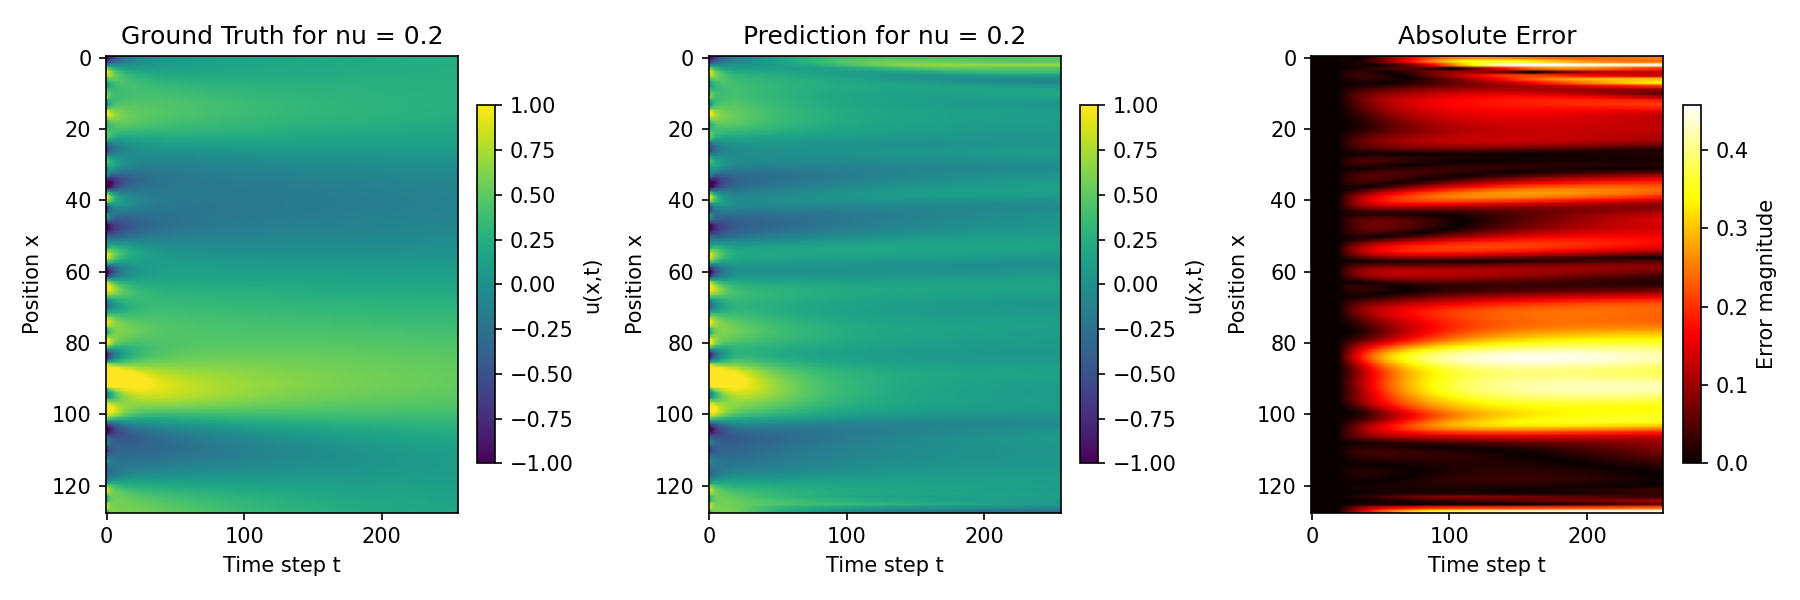
\includegraphics[width=0.55\textwidth]{images/TCAN/trajectory_epoch_0_nu0.2.png}
%     {\tiny Epoch 0}

%     \vspace{0.3cm}
%     \centering
%     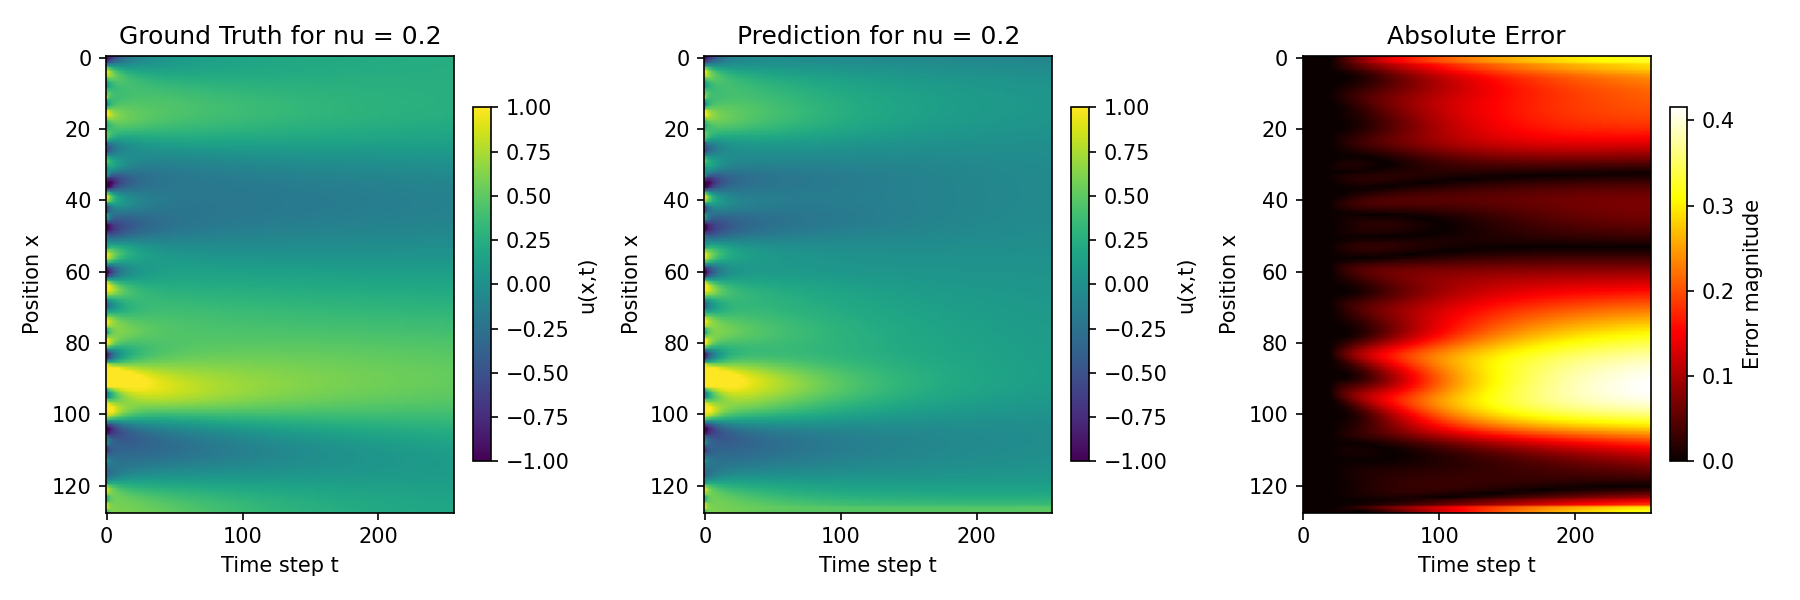
\includegraphics[width=0.55\textwidth]{images/TCAN/trajectory_epoch_40_nu0.2.png}
%     {\tiny Epoch 40}
  
%   \vspace{0.3cm}
%   \centering
%   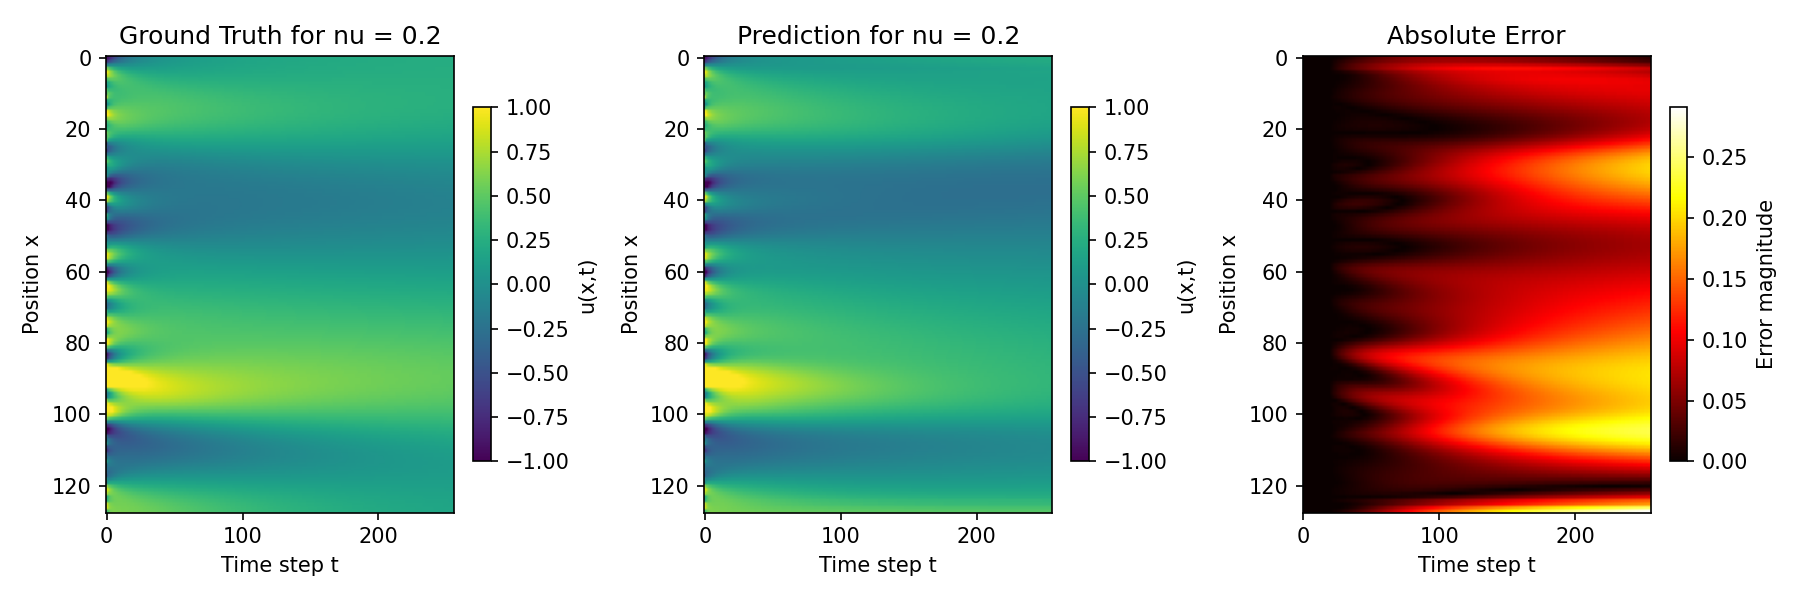
\includegraphics[width=0.55\textwidth]{images/TCAN/trajectory_epoch_80_nu0.2.png}
%   {\tiny Epoch 80}
% \end{frame}

\section{TCAN Model}

\begin{frame}{Why TCAN? Model Selection}

  \begin{block}{Three candidate architectures evaluated}
    \begin{center}
    \small
    \begin{tabular}{lccc}
      \toprule
      Architecture & Rel.\ $L^2$ ($s$=256) & Stable rollout & Resolution-robust \\
      \midrule
      CNN (ConvNet)    & 0.062 & short  & $\times$ \\
      Transformer      & 0.031 & medium & \checkmark \\
      \textbf{TCAN}   & \textbf{0.019} & \textbf{long} & \checkmark \\
      \bottomrule
    \end{tabular}
    \end{center}
  \end{block}

  \begin{columns}
    \begin{column}{0.48\textwidth}
      \begin{block}{Why not pure CNN?}
        \begin{itemize}
          \item No temporal context beyond local window
          \item Cannot capture long-range correlations in time
          \item Degrades rapidly at shock regimes
        \end{itemize}
      \end{block}
    \end{column}
    \begin{column}{0.48\textwidth}
      \begin{block}{Why not pure Transformer?}
        \begin{itemize}
          \item Quadratic attention cost over long sequences
          \item Lacks inductive spatial bias
          \item More parameters for same accuracy
        \end{itemize}
      \end{block}
    \end{column}
  \end{columns}

  \vspace{0.3em}
  \begin{block}{TCAN advantage}
    \textbf{Local} temporal convolution captures fast-changing dynamics efficiently;
    \textbf{global} causal attention integrates long-range temporal context.
    The combination yields better accuracy with fewer parameters.
  \end{block}

\end{frame}

\begin{frame}{TCAN: Model Definition}

  \begin{columns}
    \begin{column}{0.54\textwidth}
      \textbf{TCAN} = Temporal Convolutional Attention Network
      \begin{itemize}
        \item Feed-forward \textbf{autoregressive} model
        \item Operates directly on the grid $f_t = [u(x_1,t),\ldots,u(x_N,t)]$
        \item Controller in the NFTM framework
      \end{itemize}

      \vspace{0.4em}
      \textbf{Continuous Field}
      \begin{itemize}
        \item $f_t \in \mathbb{R}^N$: PDE snapshot at time $t$
        \item \textbf{Input}: window $[f_{t-W+1},\ldots,f_t]$, shape $(B,W,N)$
        \item \textbf{Output}: $\hat{f}_{t+1}$, shape $(B,1,N)$
      \end{itemize}

      \vspace{0.4em}
      \textbf{Viscosity conditioning} (FiLM)
      \begin{itemize}
        \item $\nu$ encoded as an embedding $\mathbf{e}_\nu \in \mathbb{R}^{d}$
        \item Modulates features: $\mathbf{h}' = \gamma(\mathbf{e}_\nu)\cdot\mathbf{h} + \beta(\mathbf{e}_\nu)$
        \item Enables generalisation across unseen $\nu$ values
      \end{itemize}
    \end{column}

    \begin{column}{0.43\textwidth}
      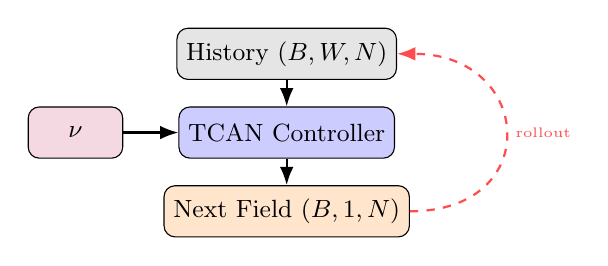
\begin{tikzpicture}[node distance=1.0cm, font=\small,
          box/.style={draw, rounded corners, minimum width=2.3cm,
                      minimum height=0.65cm, text centered}]
        \node[box, fill=gray!20]   (hist) {History $(B,W,N)$};
        \node[box, fill=blue!20,   below of=hist] (tcan) {TCAN Controller};
        \node[box, fill=orange!20, below of=tcan] (next) {Next Field $(B,1,N)$};
        \draw[-Latex,thick] (hist) -- (tcan);
        \draw[-Latex,thick] (tcan) -- (next);
        \draw[-Latex,dashed,red!70,thick] (next.east)
          to[out=0,in=0,looseness=2.2]
          node[right,font=\tiny]{rollout} (hist.east);
        % nu input
        \node[box, fill=purple!15, left=0.7cm of tcan, minimum width=1.2cm] (nu) {$\nu$};
        \draw[-Latex,thick] (nu) -- (tcan);
      \end{tikzpicture}
    \end{column}
  \end{columns}

\end{frame}

\begin{frame}{TCAN Architecture: Step by Step}

  \begin{columns}
    \begin{column}{0.42\textwidth}
      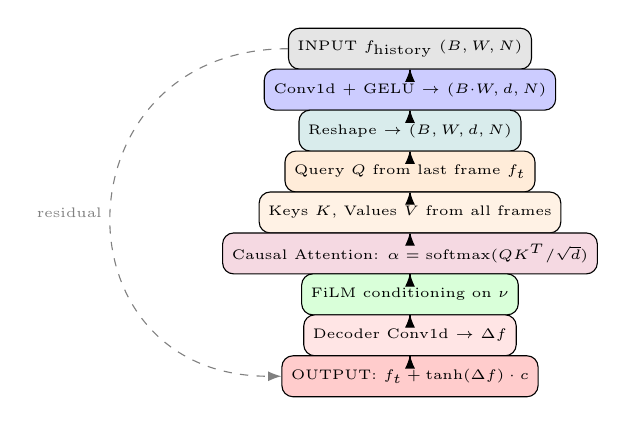
\begin{tikzpicture}[node distance=0.52cm, font=\tiny,
          blk/.style={draw, rounded corners, minimum width=2.4cm,
                      minimum height=0.52cm, text centered}]
        \node[blk, fill=gray!20]   (inp)  {INPUT $f_\text{history}$ $(B,W,N)$};
        \node[blk, fill=blue!20,   below of=inp]  (emb)  {Conv1d + GELU $\to$ $(B{\cdot}W, d, N)$};
        \node[blk, fill=teal!15,   below of=emb]  (feat) {Reshape $\to$ $(B, W, d, N)$};
        \node[blk, fill=orange!15, below of=feat] (q)    {Query $Q$ from last frame $f_t$};
        \node[blk, fill=orange!10, below of=q]    (kv)   {Keys $K$, Values $V$ from all frames};
        \node[blk, fill=purple!15, below of=kv]   (attn) {Causal Attention: $\alpha = \mathrm{softmax}(QK^T/\sqrt{d})$};
        \node[blk, fill=green!15,  below of=attn] (film) {FiLM conditioning on $\nu$};
        \node[blk, fill=red!10,    below of=film] (dec)  {Decoder Conv1d $\to$ $\Delta f$};
        \node[blk, fill=red!20,    below of=dec]  (out)  {OUTPUT: $f_t + \tanh(\Delta f)\cdot c$};
        \foreach \a/\b in {inp/emb, emb/feat, feat/q, q/kv, kv/attn, attn/film, film/dec, dec/out}
          \draw[-Latex] (\a) -- (\b);
        \draw[-Latex, dashed, gray] (inp.west)
          to[out=180,in=180,looseness=1.8]
          node[left,font=\tiny]{residual} (out.west);
      \end{tikzpicture}
    \end{column}

    \begin{column}{0.55\textwidth}
      \small
      \begin{itemize}
        \item \textbf{Conv1d + GELU}: each frame $f_t \in \mathbb{R}^N$ embedded into $d=32$ features; kernel size 3, causal padding.
        \item \textbf{Query/Key/Value}: $1\times1$ convolutions applied independently; $Q$ from last frame only (causal).
        \item \textbf{Causal Attention} per spatial position $n$:
          \[
            \alpha_{w,n} = \mathrm{softmax}_w\!\left(\frac{QK^T}{\sqrt{d}}\right)_n
          \]
        \item \textbf{FiLM conditioning}: $\nu$ projected to $\gamma, \beta \in \mathbb{R}^d$; features modulated as $\gamma \cdot h + \beta$.
        \item \textbf{Decoder}: Conv1d $\to$ scalar correction $\Delta f$.
        \item \textbf{Residual + clip}: $\hat{f}_{t+1} = f_t + \tanh(\Delta f) \cdot c$ where clipping constant $c=0.1$ ensures training stability.
      \end{itemize}
    \end{column}
  \end{columns}

\end{frame}

\begin{frame}{TCAN Training Procedure}

  \begin{columns}
    \begin{column}{0.50\textwidth}
      \begin{block}{Loss function}
        Combined \textbf{relative $L^2$} + \textbf{spatial gradient} loss:
        \[
          \mathcal{L} = \underbrace{\frac{\|\hat{f} - f\|_2}{\|f\|_2}}_{\text{rel-}L^2}
                      + \;0.1\cdot\underbrace{\|\nabla_x \hat{f} - \nabla_x f\|_2^2}_{\text{gradient loss}}
        \]
        Gradient loss penalises errors at sharp spatial features (shocks).
      \end{block}

      \begin{block}{Curriculum rollout}
        Rollout depth increases with training progress:
        \begin{itemize}
          \item Epochs $0$--$40\%$: depth $= 8$
          \item Epochs $40\%$--$75\%$: depth $= 16$
          \item Epochs $75\%$--$100\%$: depth $= T - W$ (full)
        \end{itemize}
        Prevents gradient explosion early; improves long-horizon accuracy later.
      \end{block}
    \end{column}

    \begin{column}{0.47\textwidth}
      \begin{block}{Optimiser \& regularisation}
        \begin{itemize}
          \item \textbf{Optimiser}: AdamW, lr $= 10^{-3}$, weight decay $10^{-4}$
          \item \textbf{Scheduler}: CosineAnnealingLR over full training
          \item \textbf{Gradient clipping}: max norm $= 1.0$
          \item \textbf{Input noise}: $\sigma = 0.01 \cdot \min(1, \text{epoch}/50\%)$ added to history window during training
          \item \textbf{Teacher forcing}: with probability $0.1$ during rollout (early epochs only), ground-truth frame used instead of prediction
        \end{itemize}
      \end{block}
    \end{column}
  \end{columns}

\end{frame}

\begin{frame}{TCAN Results: Qualitative}

  \begin{block}{Space-time predictions at different training epochs ($\nu = 0.2$)}
    \begin{itemize}
      \item \textbf{Epoch 0}: random initialisation; large structured error across all time steps.
      \item \textbf{Epoch 40}: model learns global advection dynamics; error substantially reduced.
      \item \textbf{Epoch 80}: prediction closely matches ground truth; residual error concentrated at sharp gradients.
    \end{itemize}
  \end{block}

  \vspace{0.3em}

  \begin{block}{Quantitative: relative $L^2$ across resolutions}
    \begin{center}
    \small
    \begin{tabular}{lcccc}
      \toprule
      Method & $s=85$ & $s=141$ & $s=211$ & $s=421$ \\
      \midrule
      FNO            & \textbf{0.0108} & \textbf{0.0109} & \textbf{0.0109} & \textbf{0.0098} \\
      \textbf{TCAN}  & -- & -- & -- & -- \\
      \bottomrule
    \end{tabular}
    \end{center}
    \small (Fill in your measured TCAN values above.)
  \end{block}

\end{frame} % Alex
% \input{sections/Transformers.tex} % Samuel
% \input{sections/Hypernetwork_Brain_Architecture.tex}
\section{2D Model Approach}
\begin{secframe}
\textbf{2D model approach}
\end{secframe} % Samuel
\section{Conclusions}
\begin{frame}
\textbf{Conclusions}
\end{frame} % Lucia



%%%%%%%%%%%%%%%%%%%%%%%%%%%%%%%%%%%%
% EXEMPLE SLIDES
%%%%%%%%%%%%%%%%%%%%%%%%%%%%%%%%%%%%

% \section{First section}

%     \begin{frame}{First section}
%         In this slide, some important text will be
%         \alert{highlighted} because it's important.
%         Here an ordered list:
%         \begin{enumerate}
%             \item First item
%             \item Second item
%         \end{enumerate}
%         Here an unordered list: 
%         \begin{itemize}
%             \item One item
%             \item Another item
%         \end{itemize}
%     \end{frame}
    
% \section{Second section}

%     \begin{frame}{Second section}
%         \begin{block}{Block}
%             Sample text in a normal block
%         \end{block}
   
%         \begin{alertblock}{Alert block}
%             Sample text in an alert block
%         \end{alertblock}    
        
%          \begin{example}
%             Sample text for an example
%         \end{example}
%     \end{frame}

    
%     \begin{emptyframe}
%         Thank you!
%     \end{emptyframe}

%     \appendix

%     \begin{frame}{Backup slide}
%         Some additional content
%     \end{frame}
    
\end{document}